% genome res: 2-12 printed pages, max of 50000 characters (~10000 words) + 4-6 figures, max abstract length 250 words
\documentclass{article}
\usepackage[hscale=0.7,vscale=0.8]{geometry}
\usepackage{microtype}
\usepackage[utf8]{inputenc}
\usepackage[T1]{fontenc}
\usepackage{graphicx}
\usepackage{xr-hyper}
\usepackage[hidelinks]{hyperref}
\usepackage[dvipsnames]{xcolor}
\usepackage[htt]{hyphenat}
\usepackage{ellipsis}
\usepackage{amsmath}
\usepackage{amsthm}
\usepackage{amssymb}
\usepackage{mathabx}
\usepackage{algorithm}
\usepackage{algpseudocode}
\usepackage{listings}
\usepackage{authblk}
\newcommand{\todo}[1]{\textbf{\textsc{\textcolor{red}{(TODO: #1)}}}}
\lstset{breaklines=true, basicstyle=\small\ttfamily, columns=flexible}
\newcommand{\Break}{\State \textbf{break} }
\newcommand\CONDITION[2]%
  {\begin{tabular}[t]{@{}l@{}l@{}}
     #1&\\ \phantom{and} #2
   \end{tabular}%
  }
\algdef{SE}[MIF]{MultiLineIf}{MultiLineEndIf}[1]%
  {\algorithmicif\ \CONDITION{#1}{\ \algorithmicthen}}%
  {\algorithmicend\ \algorithmicif}% thanks to https://tex.stackexchange.com/a/329272
\algnewcommand{\LineComment}[1]{\(\triangleright\) #1}
\usepackage{rotating}
\usepackage{booktabs}
\usepackage[labelformat=simple]{subfig}
\usepackage[font=small,labelfont=bf]{caption}
\usepackage{seqsplit}
\usepackage{multirow}
\input{ushyphex.tex}
% define new ref commands so that there isn't a wrap / page break between e.g. "Table" and "2".
\newcommand{\tabref}[1]{Table~\ref{#1}}
\newcommand{\figref}[1]{Figure~\ref{#1}}
\newcommand{\secref}[1]{Section~\ref{#1}}
\newcommand{\algoref}[1]{Algorithm~\ref{#1}}
\newcommand{\beginsupplement}{%
        \setcounter{table}{0}
        \renewcommand{\thetable}{S\arabic{table}}%
        \setcounter{figure}{0}
        \renewcommand{\thefigure}{S\arabic{figure}}%
        \setcounter{algorithm}{0}
        \renewcommand{\thealgorithm}{S\arabic{algorithm}}%
}

% make the subfloat labels look like A, B instead of a, b
\renewcommand{\thesubfigure}{\Alph{subfigure}}

% Wizardry for supplementary xrefs
\makeatletter
\newcommand*{\addFileDependency}[1]{% argument=file name and extension
  \typeout{(#1)}
  \@addtofilelist{#1}
  \IfFileExists{#1}{}{\typeout{No file #1.}}
}
\makeatother
\newcommand*{\myexternaldocument}[1]{%
    \externaldocument{#1}%
    \addFileDependency{#1.tex}%
    \addFileDependency{#1.aux}%
}
\newcommand{\code}[1]{\texttt{#1}}
\myexternaldocument{supplement}

\title{Progressive Cactus: a multiple-genome aligner for the thousand-genome era}
\author[1]{Joel Armstrong}
\author[1]{Glenn Hickey}
\author[1]{Mark Diekhans}
\author[1]{Ian T. Fiddes}
\author[1]{Alden Deran}
\author[2,12,5]{Qi Fang}
\author[2,12,3]{Duo Xie}
\author[2,12,4]{Shaohong Feng}
\author[5]{Josefin Stiller}
\author[6]{Diane Genereux}
\author[6]{Jeremy Johnson}
\author[7]{Voichita Dana Marinescu}
\author[1]{David Haussler}
\author[6]{Jessica Alföldi}
\author[6,7]{Kerstin Lindblad-Toh}
\author[6,8]{Elinor Karlsson}
\author[9,10]{Erich D. Jarvis}
\author[2,4,5,11]{Guojie Zhang \thanks{Corresponding author. Email: \href{mailto:guojie.zhang@bio.ku.dk}{guojie.zhang@bio.ku.dk}}}
\author[1]{Benedict Paten\thanks{Corresponding author. Email: \href{mailto:bpaten@ucsc.edu}{bpaten@ucsc.edu}}}
\affil[1]{UC Santa Cruz Genomics Institute, UC Santa Cruz, Santa Cruz, CA 95060, USA}
\affil[2]{China National GeneBank, BGI–Shenzhen, Shenzhen 518083, China}
\affil[12]{BGI-Shenzhen, Beishan Industrial Zone, Shenzhen 518083, China}
\affil[5]{Section for Ecology and Evolution, Department of Biology, University of Copenhagen, DK-2100 Copenhagen, Denmark}
\affil[3]{University of Chinese Academy of Sciences, Beijing 100049, China}
\affil[4]{State Key Laboratory of Genetic Resources and Evolution, Kunming Institute of Zoology, Chinese Academy of Sciences, Kunming 650223, China}
\affil[6]{Broad Institute of Harvard and Massachusetts Institute of Technology (MIT), 7 Cambridge Center, Cambridge, Massachusetts 02142, USA}
\affil[7]{Science for Life Laboratory, Department of Medical Biochemistry and Microbiology, Uppsala University, Box 582, SE-751 23 Uppsala, Sweden}
\affil[8]{Program in Molecular Medicine, University of Massachusetts Medical School, Worcester, MA 01655, USA}
\affil[9]{Laboratory of Neurogenetics of Language, The Rockefeller University, NY, USA}
\affil[10]{Howard Hughes Medical Institute, Chevy Chase, MD, USA}
\affil[11]{Center for Excellence in Animal Evolution and Genetics, Chinese Academy of Sciences, Kunming, 650223, China}
\setcounter{Maxaffil}{0}
\renewcommand\Affilfont{\itshape\small}
\begin{document}
\maketitle
\begin{abstract}
Cactus, a reference-free multiple genome alignment program, has been shown to be highly accurate, but the existing implementation scales poorly with increasing numbers of genomes, and struggles in regions of highly duplicated sequence. We describe progressive extensions to Cactus to create Progressive Cactus. Progressive Cactus enables reference-free alignment of tens to thousands of large vertebrate genomes while maintaining high alignment quality. We describe results from an alignment of over 600 amniote genomes, which is to our knowledge the largest multiple vertebrate genome alignment yet created. Further, we show improvements in orthology resolution leading to downstream improvements in annotation.
\end{abstract}
%<*cactusPaperMainText>
\section{Introduction}
New genome assemblies have been arriving at a rapidly increasing pace, thanks to decreases in sequencing costs and improvements in third-generation sequencing technologies~\cite{pacbioSequencing, supernovaHumans, nanoporeSequencing}. For example, the number of vertebrate genome assemblies currently in the NCBI database~\cite{genbankAssembly} has increased by over 50\% in just the past year (to 1485 assemblies as of July 2019). The Vertebrate Genome Project, Genome 10K~\cite{genome10k}, the Earth BioGenome Project~\cite{Lewin4325}, the Bird 10K project~\cite{b10kProjectAnnounce}, and the 200 Mammals project~\cite{200mPerspectivesPiece}, among others, aim to release hundreds of high-quality assemblies of previously unsequenced genomes in the next year, and thousands over the next decade.

In addition to this influx of assemblies from different species, new human \emph{de novo} assemblies~\cite{nanoporeHumanAssembly} are being produced, which enable analysis of not just small polymorphisms, but also complex, large-scale structural differences between human individuals and haplotypes. This coming era and its unprecedented amount of data offers the opportunity to unlock many insights into genome evolution, but also presents challenges in adapting our analysis methods to meet the increased scale.

% genome alignment is necessary to analyze these genomes.
Often we want to make use of these assemblies to conduct analyses like species-tree inference~\cite{mpEst,astral}, comparative annotation~\cite{cat,augustusCGP}, or constraint detection~\cite{phast,siPhy}. All of these require comparing an assembly against one or more other assemblies. This involves creating a mapping from each region of each genome to a corresponding region in each other genome, taking into account the possibility of complex rearrangements: this is the problem of creating a \emph{genome alignment}~\cite{genomeAlignmentAnnotationReview}. Genome aligners are one of the most fundamental tools used in comparative genomics, but since the problem is difficult, different aligners frequently give different results~\cite{earl2014alignathon}, 
%% I am omitting this here ,because it makes us all sound very bad, also we raise this issue later
%(for example, some aligners disagreed on as many as 72\% of their aligned pairs in the flies dataset of the Alignathon~\cite{earl2014alignathon})
and many intentionally limit the alignments they produce to simplify the problem. Two of the most common limitations are \emph{reference-bias}, the result of constraining a multiple alignment to only regions present in a single reference genome, and restricting the alignment to be \emph{single-copy}, which allows only a single alignment in any column in any given genome, causing the alignment to miss multiple-orthology relationships created by lineage-specific duplications. Cactus~\cite{cactusGenomeRes} is a genome alignment program which has neither of these restrictions; it is capable of generating a reference-free multiple alignment that allows detecting multiple-orthology relationships.

% introduce cactus, identify scaling problem, describe generally the fix
The version of Cactus available in 2012 performed very well in the Alignathon~\cite{earl2014alignathon}, an evaluation of genome aligners. However, the runtime of that initial iteration of Cactus scaled quadratically with the total number of bases in the alignment problem, making alignment of more than about ten vertebrate genomes completely impractical. To address these difficulties, we present fundamental changes to the Cactus process that incorporate a progressive alignment strategy~\cite{progressiveAlignment}, which changes the runtime of the alignment to scale linearly with the number of genomes. We show that the result, which we call Progressive Cactus, is an aligner that remains state-of-the-art in accuracy, and continues to lack reference bias, but which is tractable to use on hundreds to thousands of large, vertebrate-sized input genomes. Progressive Cactus has been developed over several years, and has already been successfully used as an integral component of high-profile comparative genomics projects~\cite{crocs,cheetah,gordon2016long,mousePaper,greatApes}. We describe the many innovations in Progressive Cactus that make large alignments tractable, and demonstrate this by describing a new 600-way vertebrate genome alignment of bird and mammalian genomes. 

%% I'm proposing cutting this as we don't really tackle, but will instead move to the discussion
%We demonstrate it is capable of creating useful alignments across a wide range of evolutionary distances, from intra-species alignments useful in population genetics~\cite{yeastCactusVg} to inter-species alignments spanning hundreds of millions of years of genome evolution. Because of its support for multiple-orthology relationships, it automatically supports diploid assemblies, which are becoming more common as new technologies enable phasing across long distances~\cite{pacbioZebraFinch, supernovaHumans}.

\section{Results}
\subsection{Cactus}
The new progressive Cactus pipeline is freely available and open source. The only inputs needed are a guide tree and a FASTA file for each genome assembly. 

\begin{figure}
\begin{center}
\subfloat[]{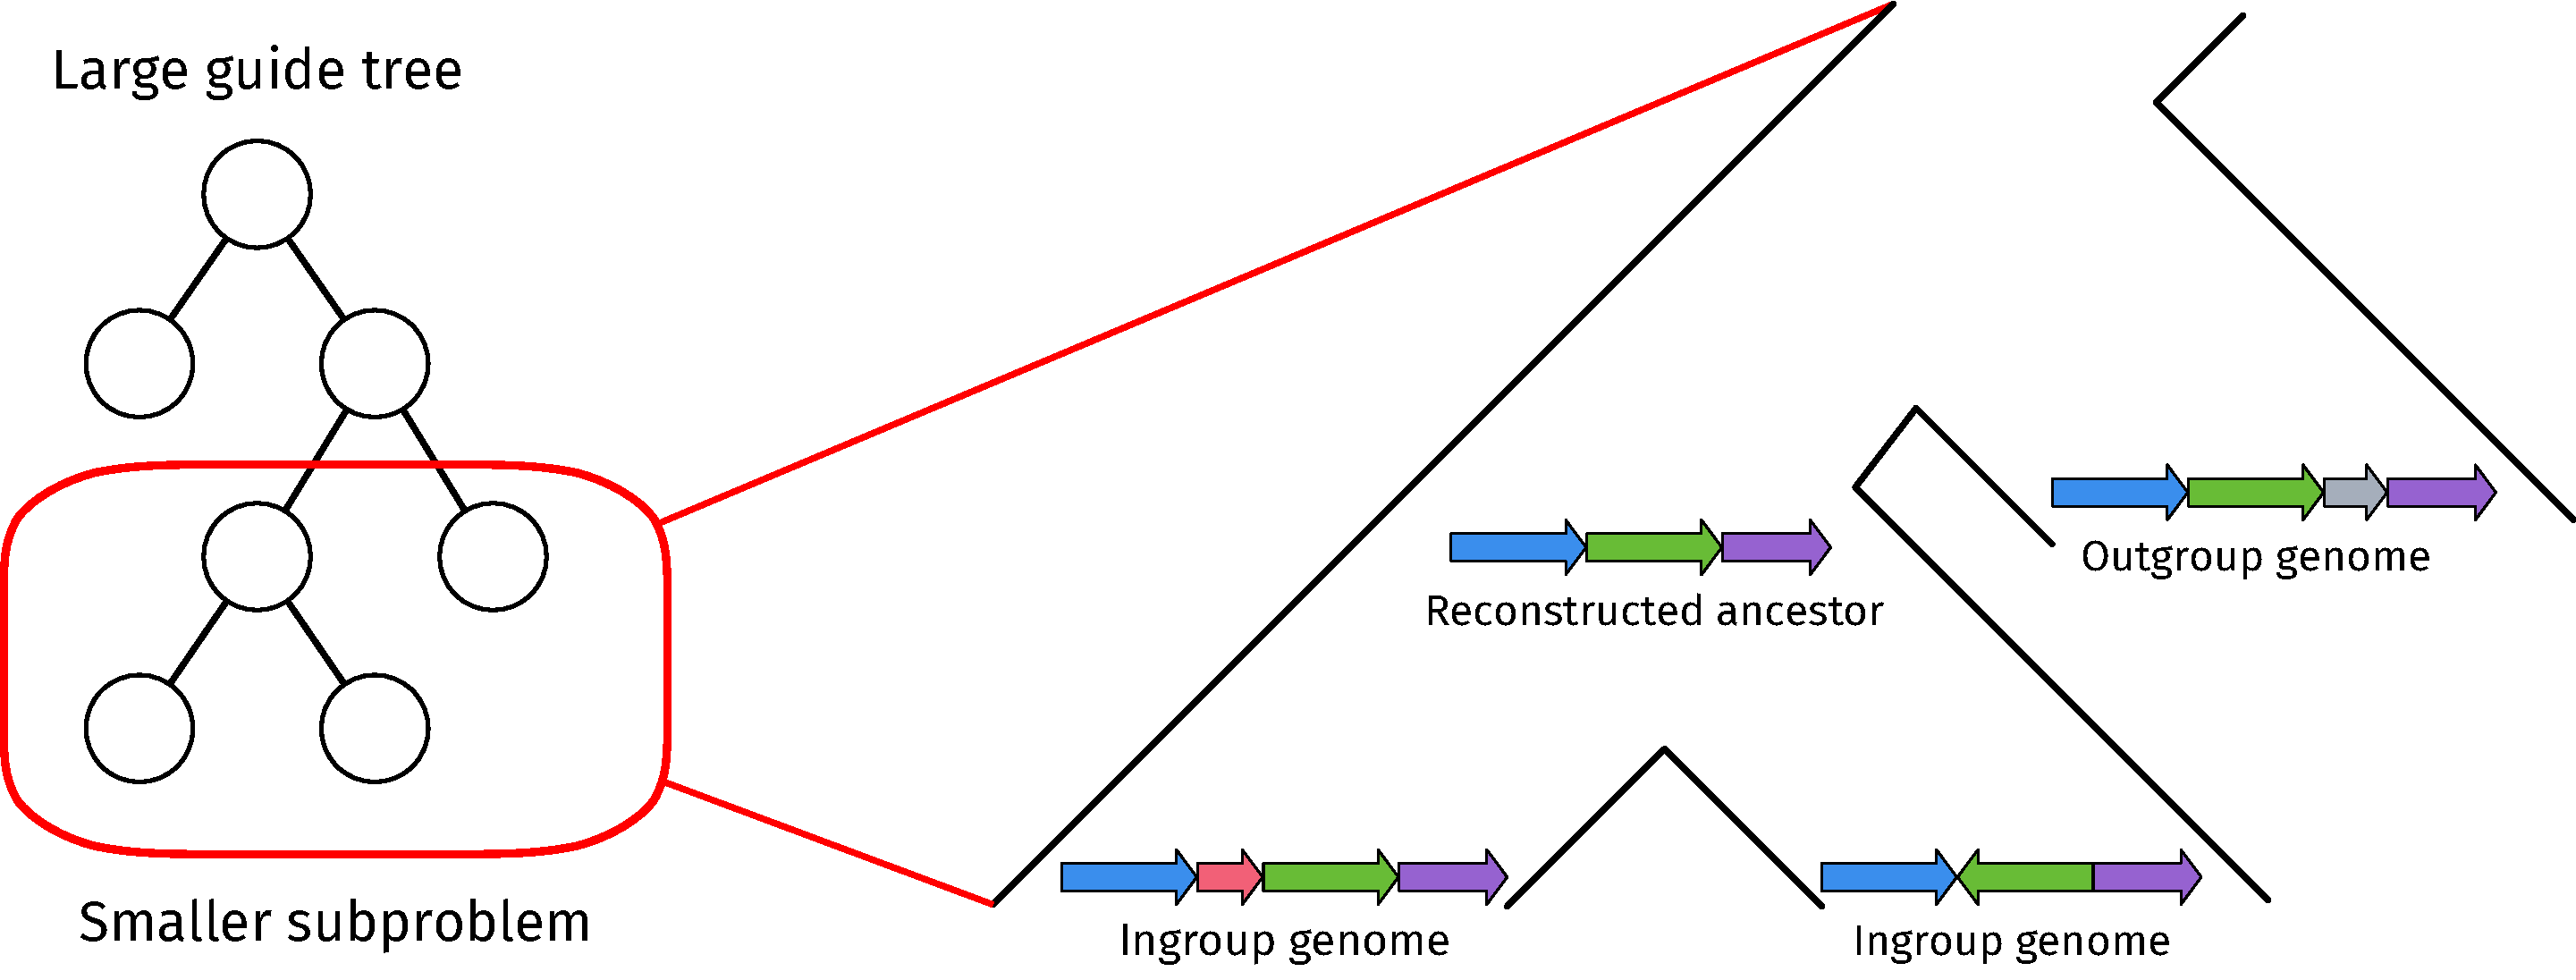
\includegraphics[width=\textwidth]{progressive-alignment-and-reconstruction}}\\
\subfloat[]{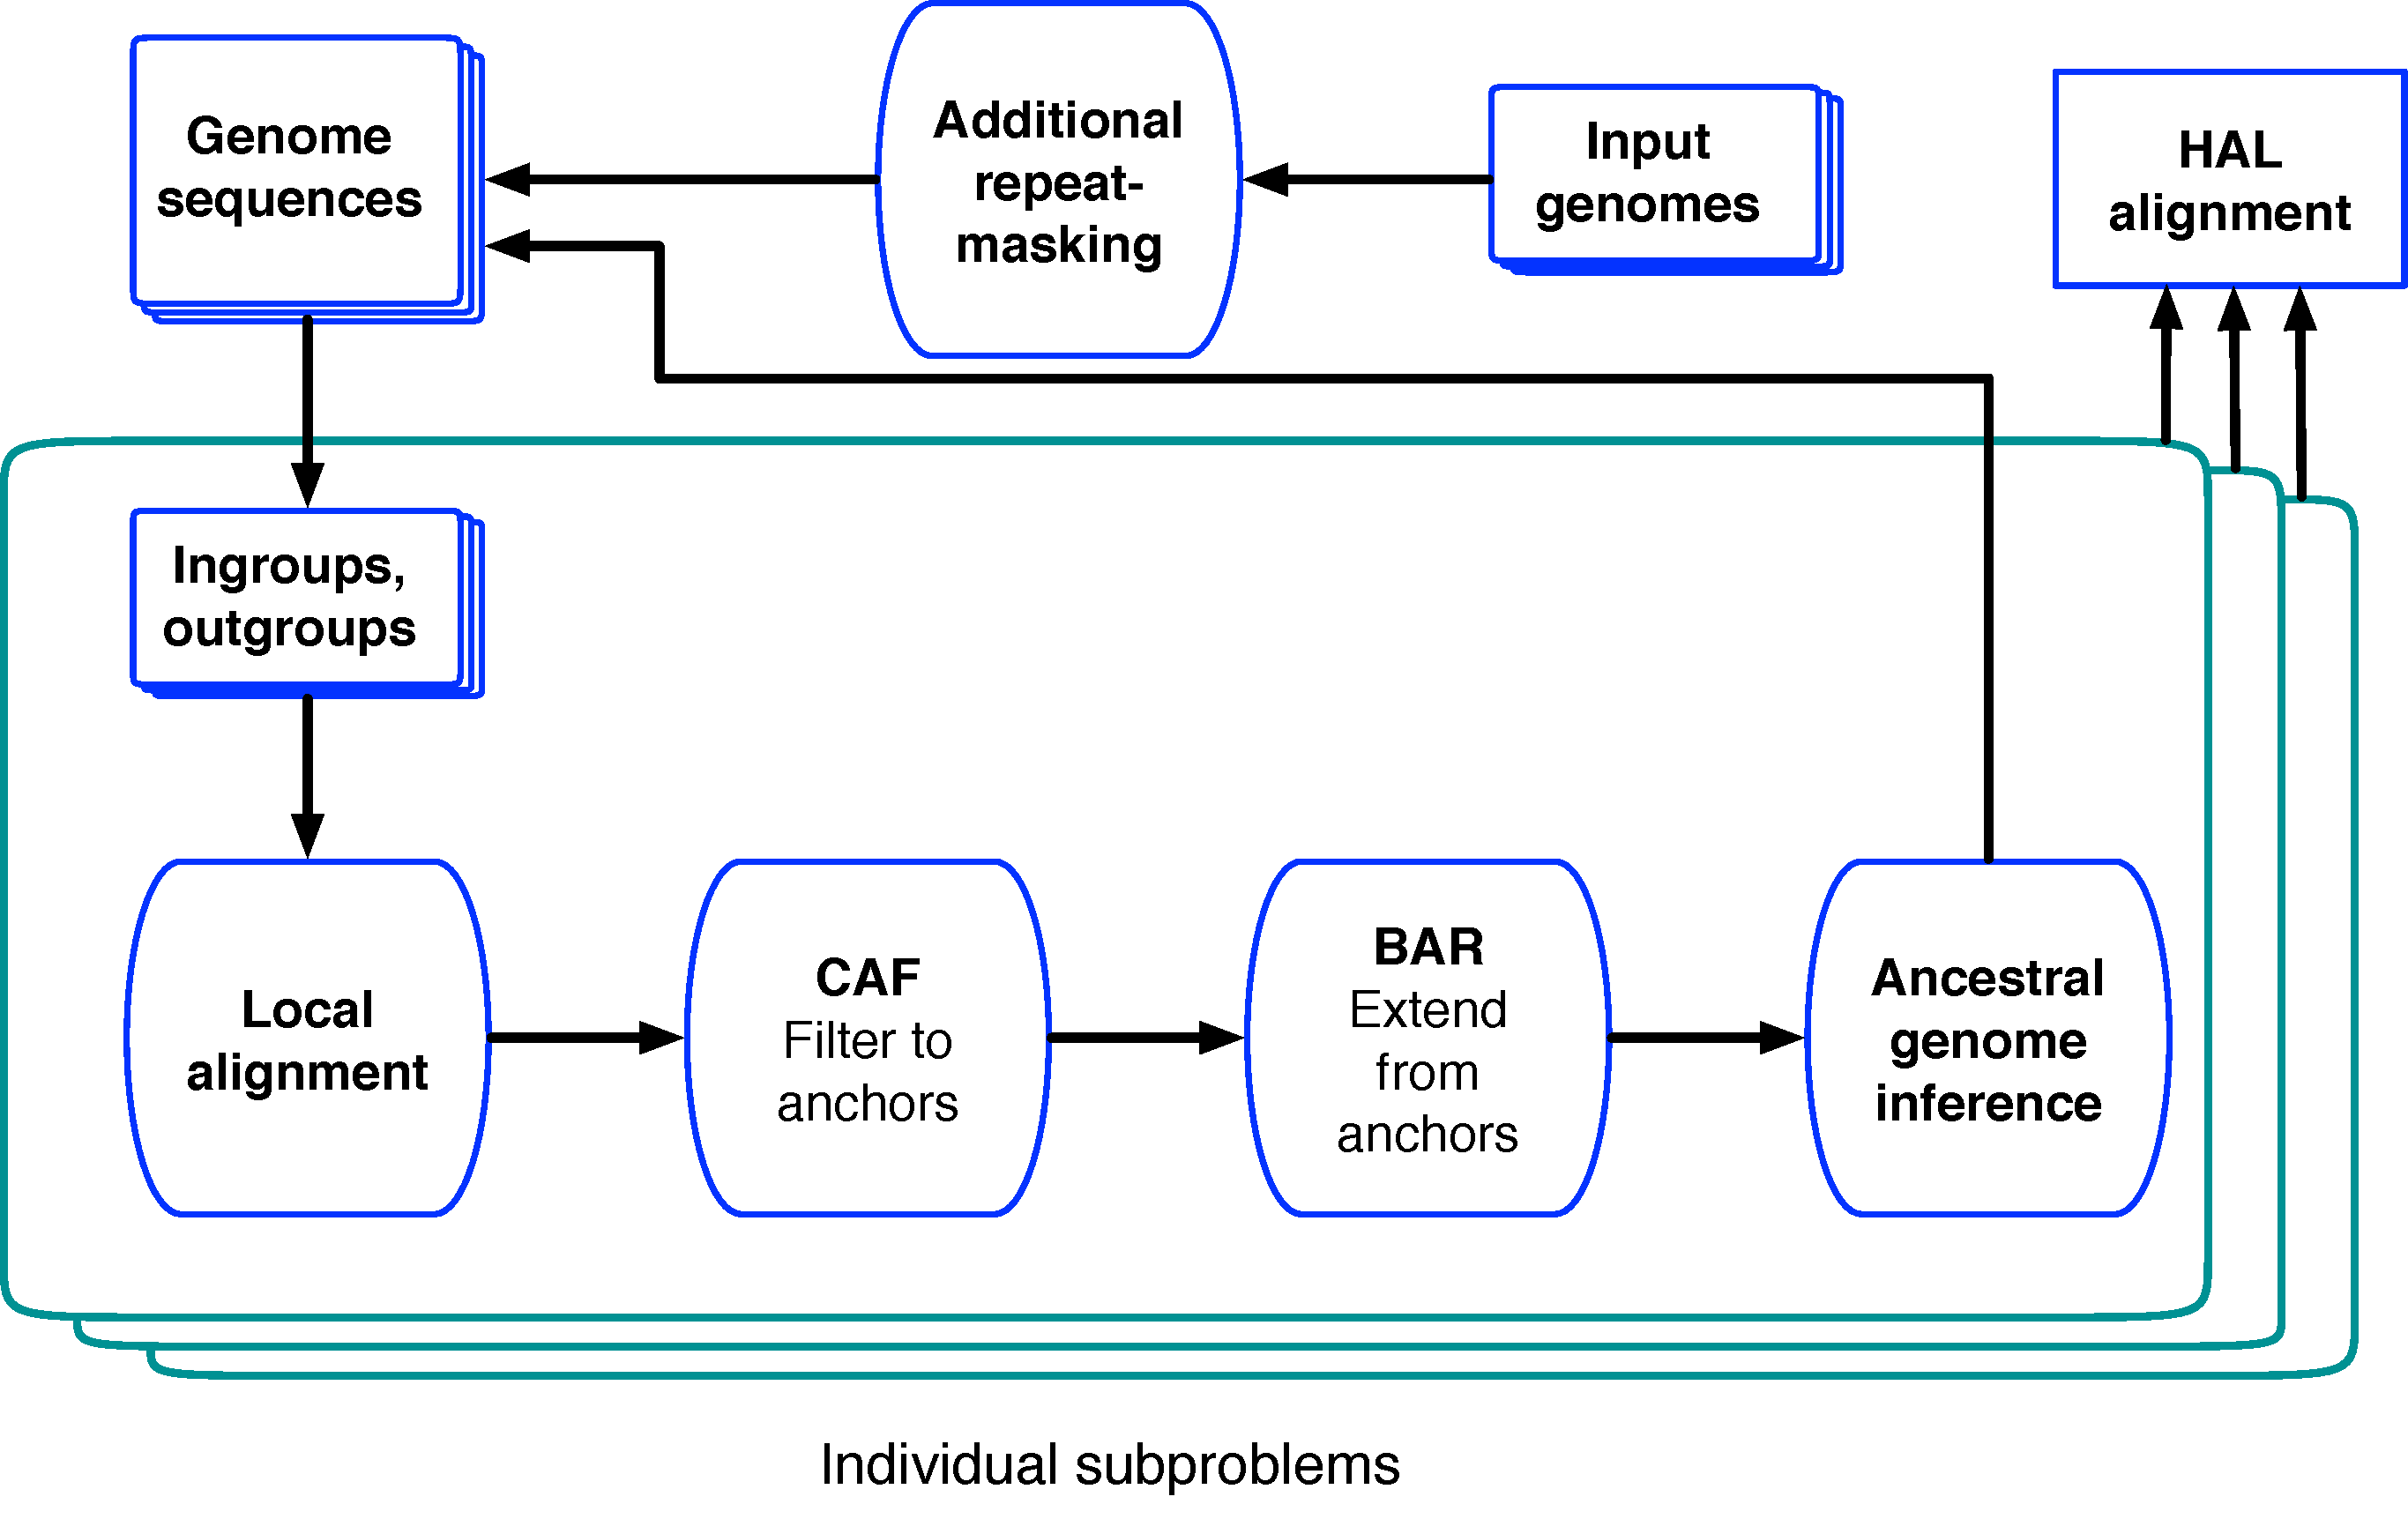
\includegraphics[width=\textwidth]{flowchart.pdf}}%
\caption[A diagram of the alignment process within Progressive Cactus]{A diagram of the alignment process within Progressive Cactus. A:\@ A large alignment problem is decomposed into many smaller subproblems using an input guide tree. Each subproblem compares a set of ingroup genomes (the children of the internal node to be reconstructed) against each other as well as a sample of outgroup genomes (non-descendants of the internal node in question). B:\@ 
This flowchart represents the phases which the overall alignment, as well as each subproblem alignment, proceeds through.
The end result is a new genome assembly representing Progressive Cactus's reconstruction of the ancestral genome, as well as an alignment between this ancestral genome and its children. After all subproblems have been completed, the parent-child alignments are combined to create the full reference-free alignment in the HAL~\cite{hal} format. }\label{fig:progressiveDiagram}
\end{center}
\end{figure}

The key innovation Progressive Cactus is to adapt the classic \emph{progressive} strategy (used in collinear multiple alignment for decades) to a whole-genome alignment setting. Progressive aligners use a \emph{guide tree} to recursively break a multiple alignment problem into many smaller sub-alignments, each of which is solved independently; the resulting sub-alignments are themselves aligned together according to the tree structure to create the final alignment. Progressive alignment has been succesfully applied to whole-genome alignment before, for example by progressiveMauve~\cite{progressiveMauve} and TBA/MULTIZ~\cite{tba}. Cactus now follows a similar strategy, with the key innovation being that Progressive Cactus implements a progressive-alignment strategy for whole-genome alignment using reconstructed ancestral assemblies as the method for combining sub-alignments. This strategy (analogous to MAVID's~\cite{mavid} strategy of using ancestral reconstruction in collinear multiple alignment) not only results in a much faster alignment runtime, but also produces ancestral reconstructions.

As a practical matter, Progressive Cactus also uses the Toil~\cite{toil} workflow framework to organize and distribute its computational tasks. Because it runs on Toil and supports container execution via Docker and Singularity~\cite{singularity}, Progressive Cactus can be run on many different environments: single machines (for small alignments), conventional HPC clusters, as well as the GCP, AWS, and Azure clouds.

\figref{fig:progressiveDiagram}A shows the overall organization of the Progressive Cactus process. The guide tree, which need not be fully resolved (binary), is used to recursively split a large alignment problem (comparing every genome to every other genome) into many small subproblems, each of which compares only a small number (usually 2--5) of genomes against one another. The purpose of each subproblem is to reconstruct an ancestral assembly at each internal node in the guide tree, as well as to generate alignments between that internal node's children and its ancestral reconstruction. The ancestral assemblies are then used as input genomes in subproblems further up the tree, while the parent-child alignments are later combined to produce the full alignment. Two sets of genomes are considered: the children of the internal node (which we call the \emph{ingroup genomes}), and a set of non-descendants of that node (the \emph{outgroup genomes}). The ingroup genomes form the core alignment relationship being established at this node. The outgroup genomes serve to answer the question of what sequence from the ingroups is also present in the ancestor (whether an indel among the ingroups is likely a deletion rather than an insertion), and in how many copies (whether a duplication predates or postdates the speciation event the node represents). The outgroups also provide information for guiding the ancestral assembly by providing order-and-orientation information, as well as base-level information when generating ancestral sequences. These genome sets are used as the input to the main subproblem workflow, which we outline below and in \figref{fig:progressiveDiagram}B, and describe in detail in \secref{sec:cactusMethods}.

Each individual subproblem follows a procedure akin to the original Cactus process. The subproblem procedure begins with a set of pairwise local alignments generated via the sensitive pairwise local-alignment program LASTZ~\cite{lastz}. These pairwise alignments are then filtered and combined into a cactus graph representing an initial multiple alignment using the CAF algorithm described in our earlier work~\cite{cactusGenomeRes}, though we note important changes to the filtering in \secref{sec:mapQ} and \secref{sec:removeRecoverableChains}. The initial alignment is refined using the BAR algorithm again described in earlier work~\cite{cactusGenomeRes} to create a more complete alignment. The ancestral assembly is then created by ordering the blocks in this final alignment and establishing a most-likely base call for each column in each block. The resulting ancestral sequence is then fed into later subproblems (unless the subproblem represents the root of the guide tree, which indicates the end of the alignment process).

\subsection{Evaluation on simulated data}

% \todo{ADD Alignathon results here - this can be the first analysis}
The Alignathon's simulated datasets \cite{earl2014alignathon} have been aligned with many competing genome aligners and have a known truth set, providing a way to compare Progressive Cactus against other genome aligners. Progressive Cactus produces alignments with higher accuracy for both simulated primate (F1 0.989) and mammal (F1 0.795) clades than any aligner that participated in the Alignathon (\tabref{tab:alignathonMammals} and \tabref{tab:alignathonPrimates}), including the original version of Cactus.


\label{sec:simulationResults}
\begin{figure}
\begin{center}
\subfloat[]{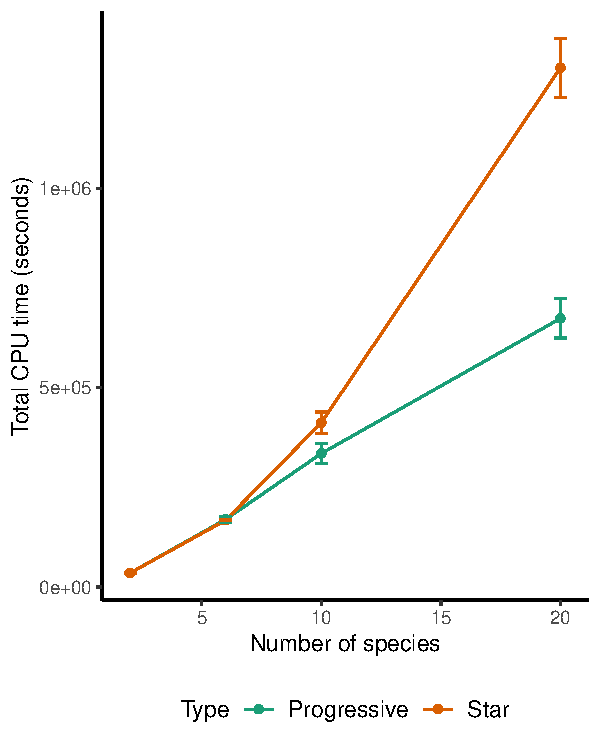
\includegraphics[width=0.5\textwidth]{evolver_runtime.pdf}}
\subfloat[]{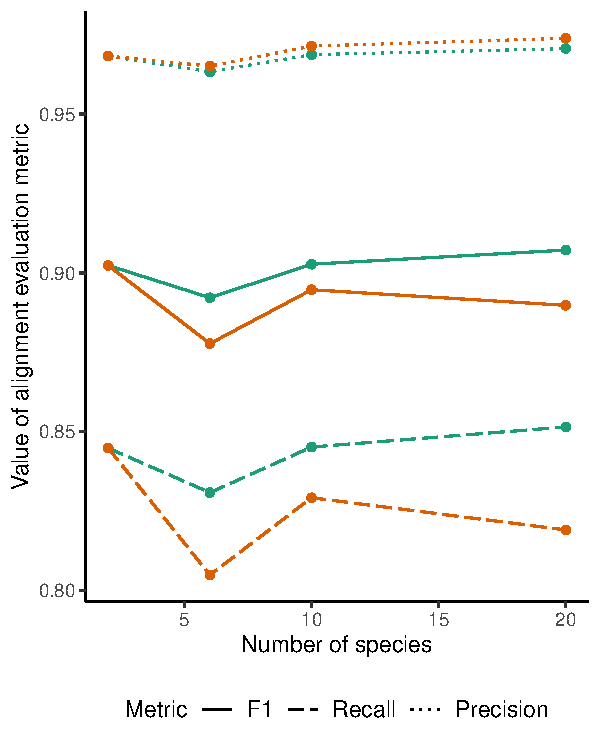
\includegraphics[width=0.5\textwidth]{evolver_combined_metrics.pdf}}
\caption[Comparison between progressive and non-progressive Cactus using results on simulated genomes]{Results from alignments of varying numbers of simulated genomes using the progressive mode of Progressive Cactus (``Progressive''), versus the mode without progressive decomposition similar to originally described in~\cite{cactusGenomeRes} (``Star''). A) The total runtime of the two alignment methods across 3 runs. Error bars show standard deviation of runtime between the runs. The runtime is nearly identical when aligning two genomes since the alignment problem is not further decomposed, but the linear scaling of the progressive mode means it is much faster with large numbers of genomes than the quadratic scaling required without progressive alignment. B) The precision, recall, and F1 score (harmonic mean of precision and recall) of aligned pairs for each alignment compared to pairs from the true alignment produced by the simulation.
}\label{fig:simulationEvaluation}
\end{center}
\end{figure}

To evaluate the improvements in quality and runtime of the alignments produced using the new progressive alignment strategy, we simulated the evolution of 20 30-megabase genomes using Evolver~\cite{evolver} along a tree of catarrhines. We ran two alignment strategies --- one using a fully-resolved binary guide tree (which takes full advantage of the new progressive mode) and one using a fully-unresolved star guide tree (which is similar to the originally published version of Cactus) --- across variously-sized subsets of genomes roughly evenly spaced throughout the catarrhine tree (\secref{sec:simulationEvaluationSupplement}). The alignments using the progressive strategy finished more quickly, with the speed improvement growing larger with increasing number of species (e.g. a 15\% reduction in runtime for 10 species and 48\% for 20 species), due to its linear runtime scaling, as opposed to the quadratic scaling of the star-tree (\figref{fig:simulationEvaluation}A). The progressive strategy is also more accurate than the star strategy (\figref{fig:simulationEvaluation}B) and maintains accuracy as the number of species (and therefore nodes in the tree) increases. 

\subsection{Effect of the guide tree}

%\todo{ADD: Analysis of how individual pairwise alignments are changed by guide tree changes}. 

\begin{table}
\begin{center}
\begin{tabular}{lrrrr}
\toprule
Guide tree & Jarvis & Prum & Consensus & Permuted \\
\midrule
Jarvis & 1 & & & \\
Prum & 0.9867 & 1 & & \\
Consensus & 0.9882 & 0.9883 & 1 & \\
Permuted & 0.9843 & 0.9822 & 0.9836 & 1 \\
\bottomrule
\end{tabular}
\end{center}
\caption[Comparison of alignment similarity between four alignments of the same 48 avian genomes with different guide trees]{Comparison of alignment similarity between four alignments of the same 48 avian genomes with different guide trees. Similarity between each pair of alignments is represented by the F1 score of aligned-pair relationships in the two alignments.}\label{tab:f1scores}
\end{table}
Since Progressive Cactus uses an input guide tree to decompose the alignment problem, the guide tree can potentially impact the resulting alignment. This could be problematic when the exact species tree relating the input set of genomes is unknown or controversial. However, we reduce any effect of the guide tree by including a great deal of outgroup information, including multiple outgroups when possible. To quantify the effect of the guide tree on a large alignment with an uncertain species tree, we created four alignments of a set of 48 avian species, which we subsetted down to a single chromosome (Chromosome 1). The avian species tree is still being actively debated~\cite{prumSpeciesTree,jarvisSpeciesTree} and there are different plausible hypotheses, making birds an excellent test case with no single clearly correct guide tree. We aligned these birds using four different guide trees: two trees that represent two different hypotheses about the avian species tree (Jarvis et al.~\cite{jarvisSpeciesTree} and Prum et al.~\cite{prumSpeciesTree}), one consensus tree between the former two trees, and one tree that was randomly permuted from the Jarvis et al. tree (\secref{sec:guideTreeSupplement}, \figref{fig:guideTreeTrees}). The four alignments were highly similar, with an average of 98.5\% of aligned pairs exactly identical between any two different alignments (\tabref{tab:f1scores}).

We further examined whether these small differences in the guide tree impact some species more than others. For any pair of these 48 species, the F1 score for aligned pairs between the Jarvis et al. based and Prum et al. based alignments was at least 0.955 (\figref{fig:jarvisPrumCompareMatrix}). As an example, the phylogenetic relationship between the species \emph{Cuculus canorus}, \emph{Chlamydotis macqueenii}, and \emph{Tauraco erythrolophus} is different in the Prum et al. based guide tree than the Jarvis et al. based guide tree (\figref{fig:jarvisPrumCompare}). The F1 score for aligned pairs within this clade between the two alignments was 0.972, lower but comparable to the score for a similar clade which had an identical phylogenetic relationship in both trees, 0.982 (for \emph{Merops nubicus}, \emph{Picoides pubescens}, and \emph{Buceros rhinoceros}).

\subsection{Effect of assembly quality on alignment}

The progressive approach we use means that the alignment between two genomes distant in the guide tree is informed by the reconstructions of the ancestral genomes along the path, which is in turn formed using data from other genomes in the tree. 
To evaluate the practical effect this has on alignments, we created two alignments of 11 boreoeutherian species, 7 of which represented either high-quality assemblies in one alignment (using modern assemblers and often long-read data) or lower-quality assemblies in the other alignment (usually using much older technologies) (\tabref{tab:assembly_quality_comparison_assemblies}). The remaining 4 assemblies were held constant to facilitate comparison between the two alignments. 
Despite alignment differences between the new and old assemblies (\tabref{tab:new_vs_old_assemblies_coverage}), the alignment between these 4 assemblies was similar between the two alignments (e.g. 0.855 Jaccard similarity between induced pairwise human-dog alignments; \figref{fig:new_vs_old_assemblies_aligned_pairs}), a level of similarity higher than seen between alignment strategies, indicating that the progressive alignment strategy can tolerate poor assemblies. Reinforcing this, comparing the induced pairwise alignments of human-dog to direct pairwise alignments computed using the established Chains and Nets pipeline~\cite{kent2003evolution}, we find the same level of Jaccard similarity for both the high and low quality assembly alignments (\figref{fig:comparisonToChainsAndNets}). With 82\% of aligned pairs in the induced pairwise Progressive Cactus alignments being found in the Chains and Nets alignment and, vice versa, 78\% of pairs in the Chains and Nets alignment being found in each Progressive Cactus alignment. Concordant results were found comparing human-mouse pairwise alignments (\figref{fig:comparisonToChainsAndNets}). 

\subsection{Adding new genomes to an existing alignment}
\begin{table}
\begin{center}
\begin{tabular}{lrrrr}
\toprule
Alignment & Precision & Recall & F1-score & CPU time \\
\midrule
Genome added to branch & 97.27\% & 88.40\% & 92.63\% & 11 h \\
Genome added to node & 97.21\% & 88.35\% & 92.57\% & 16 h \\
Full realignment of entire tree \& new genome & 97.19\% & 88.33\% & 92.55\% & 176 h \\
\bottomrule
\end{tabular}
\caption[Results of adding a new genome to an alignment of simulated genomes]{Results of adding a new genome to an alignment of simulated genomes. Precision, recall, and F1-score statistics are all of aligned pairs that contain a base of the added genome. An alignment where the genome was included initially is shown for comparison.}\label{tab:addGenomeStats}
\end{center}
\end{table}
Given the rate of arrival of new assembly versions and newly sequenced genomes, adding new information to an alignment without recomputing it from scratch is valuable, especially for large alignments where recomputing the entire alignment is often cost-prohibitive.
Progressive Cactus supports adding a new genome to an existing alignment by taking advantage of the tree structure of the progressive alignments it produces. There are three ways that a new genome can be added to an alignment, depending on its phylogenetic position relative to the existing genomes: 1) as outgroup to all the existing genomes in the alignment, 2) by being added as a new child of an existing ancestral genome in the alignment, or 3) by splitting a branch in the existing alignment, creating a new internal node and two new branches (\figref{fig:addGenomeSupp}). Progressive Cactus allows adding a new genome in any of these ways, though the details differ (\secref{sec:addingAGenomeMethods}). Assemblies can be replaced with new versions by simply deleting them and adding the new assembly in as a leaf. Adding multiple genomes is possible, either iteratively or (if the new genomes are monophyletic) by aligning together the new genomes and adding in the ancestral clade root.

We tested the effect of adding a new genome to an existing alignment using the same set of simulated catarrhine genomes as in \secref{sec:simulationResults}. To replicate the use-case of an end-user wanting to add a genome to a previously-created alignment, we generated an alignment holding out one of the 20 genomes (the crab-eating macaque), and added that genome back into the alignment by both splitting an existing branch (resulting in the same topology as a full alignment would), and by adding the macaque as a new child of an existing ancestor (creating a trifurcation which did not exist in the original tree; \secref{sec:addGenomeTestSupplement}). Both methods resulted in alignments that had accuracy deviating less than 0.1\% from the full alignment that included the macaque from the start: both addition methods as well as the full alignment achieved an F1 score of 0.926 (\tabref{tab:addGenomeStats}).

\label{sec:addGenomeTestSupplement}
\begin{figure}
\begin{center}
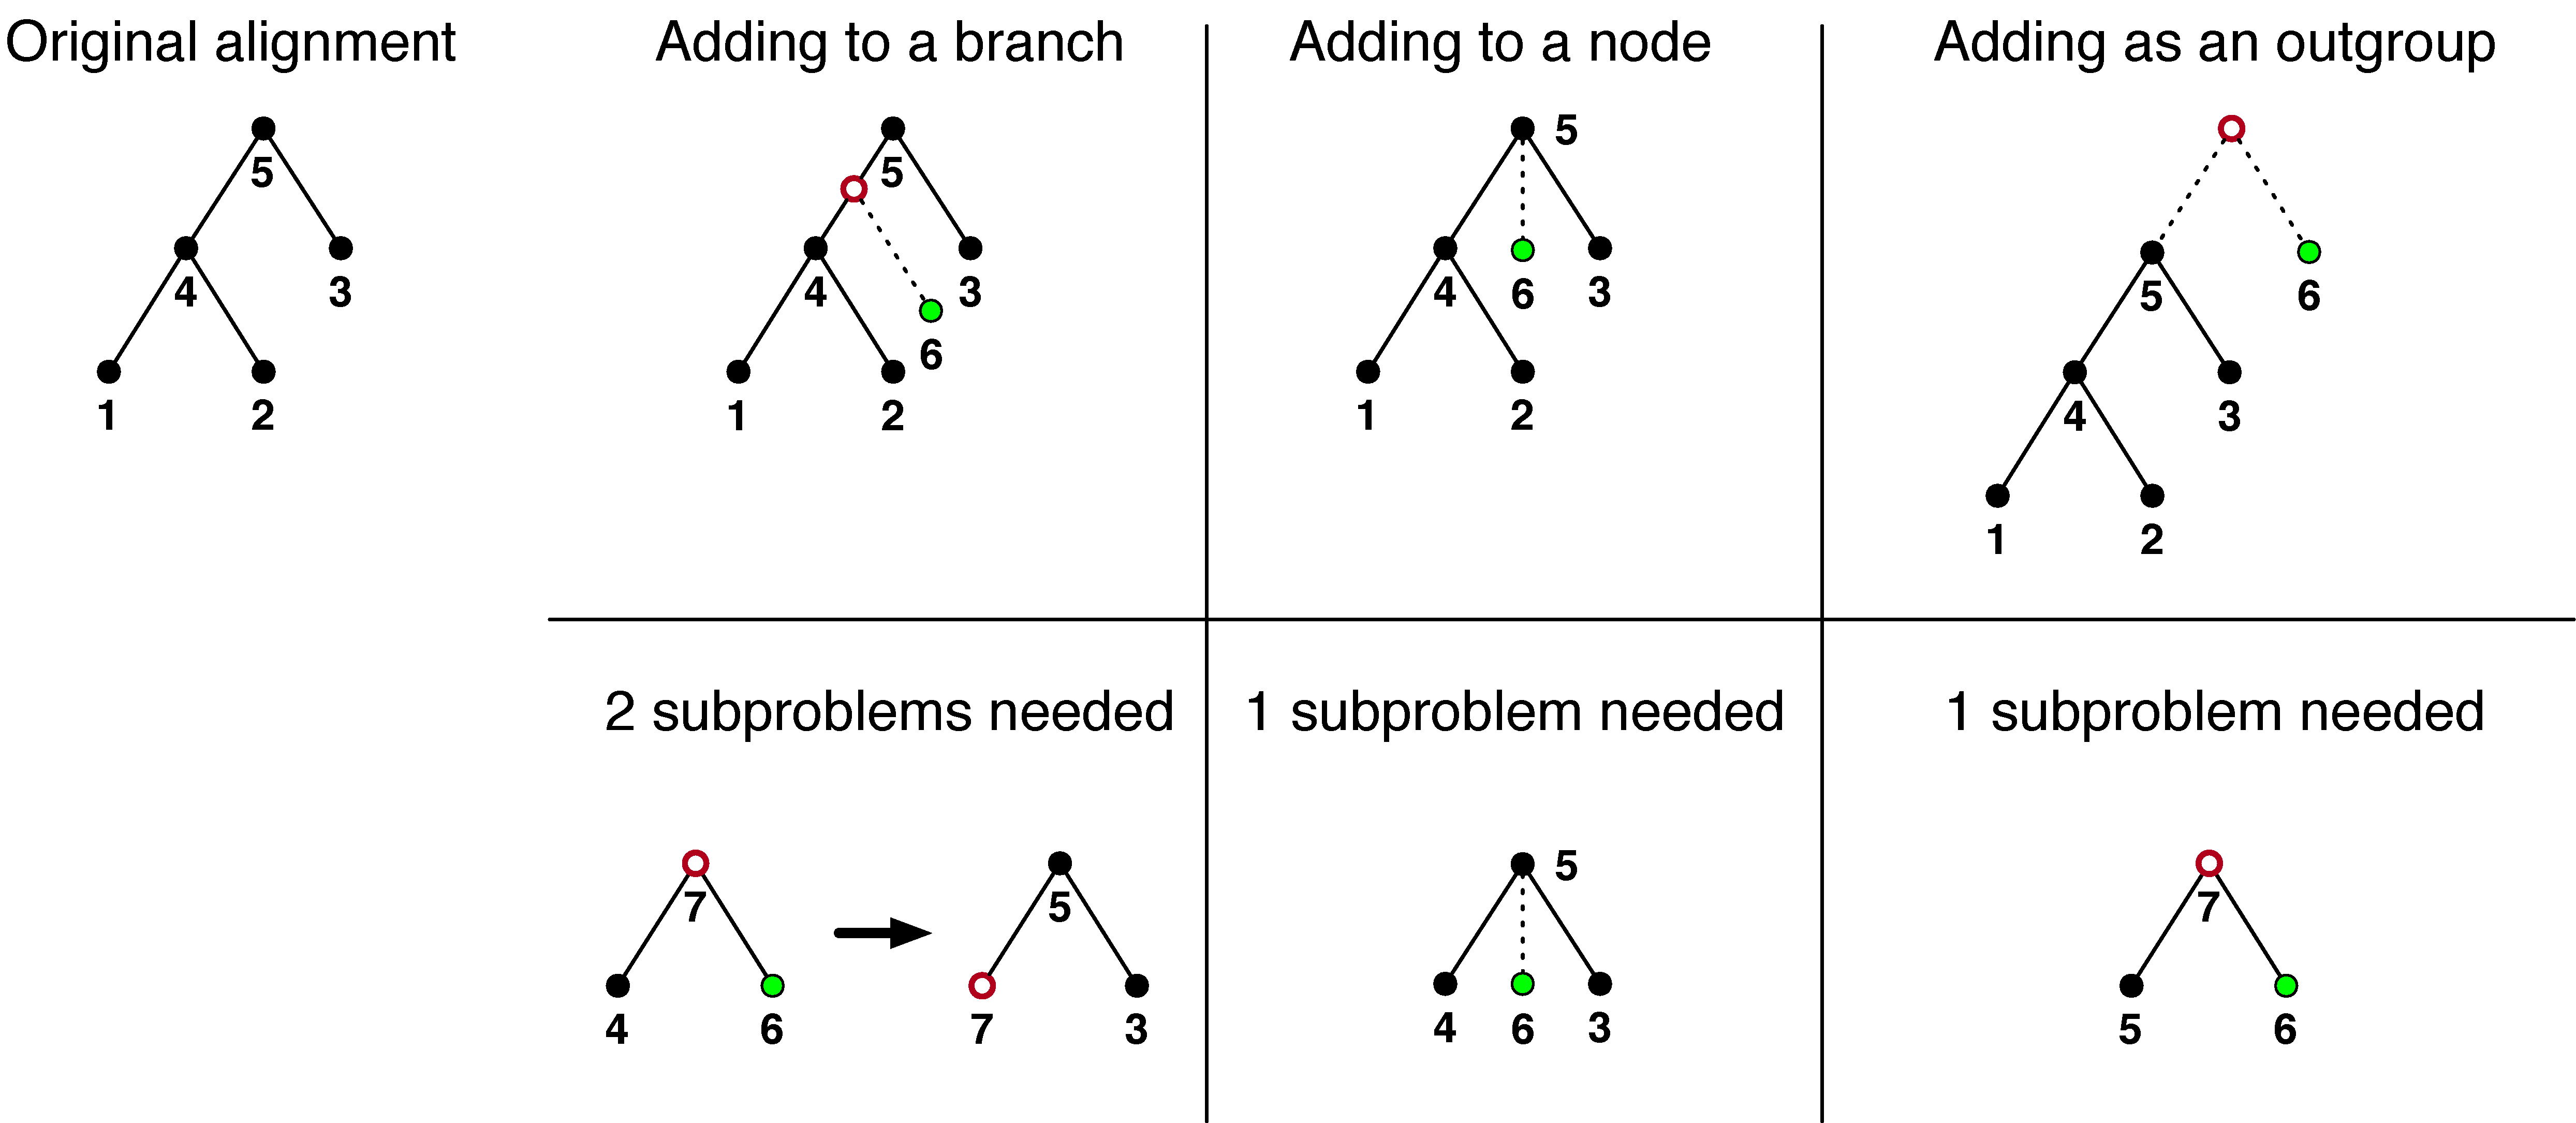
\includegraphics[width=\textwidth]{add-genome-fig}
\caption[Methods of adding a genome to a Progressive Cactus alignment]{Methods of adding a genome to a Progressive Cactus alignment. The top row shows the different ways of adding a new genome given its phylogenetic position, and the bottom row shows what subproblems would need to be computed for the new genome to be properly merged into the existing alignment. Green circles represent a new genome, and red circles represent newly reconstructed genomes.}\label{fig:addGenomeSupp}
\end{center}
\end{figure}

% Raw tree results
\subsection{Timing duplication events}
Users of a genome alignment are often interested in \emph{orthology} relationships, rather than all \emph{homology} relationships, between a set of sequences. For example, when comparing human and chimpanzee KZNF genes, providing an alignment from each gene to the over-400~\cite{kznfEvolution} homologous KZNF genes in the other genome is nigh-useless; the user is likely interested in only the orthologous copy or copies (in the case of a lineage-specific duplication) in the other genome. For this reason, Progressive Cactus alignments are capable of representing complex orthology/paralogy relationships, with an ability to display the alignment(s) labeled as orthologous, but also the option for a user to request alignments to paralogs at a customizable coalescence-time threshold. This is achieved by implicitly producing a gene tree as the alignment is built, albeit with some restrictions, namely that a duplication event is represented by multiple regions in the child(ren) aligned to a single region in the parent species. This forbids the representation of gene-tree-species-tree discordance as would occur in incomplete lineage-sorting or horizontal transfer, as well as the exact ordering of multiple duplication events along a single branch. The restricted problem we solve at each subproblem step is that each alignment block should represent all regions orthologous to a single region of the ancestral sequence, possibly multiple per species; we make no attempt to fully resolve the gene tree when multiple duplications take place along a single branch. However, this still requires resolving the timing of all duplication events to the lineages of the tree: duplicated sequences whose coalescence precedes the speciation event represented in the subproblem should be split, while those following the speciation event should be kept together.

Because it is impractical to generate maximum-likelihood trees for every block in the subproblem, Progressive Cactus relies on heuristically filtering alignments to remove paralogs before building its cactus graph. For this we developed two heuristics: a filter based on similarity to outgroup sequence, which was used in the many projects which used the beta versions of Progressive Cactus, and (more recently) a method of pre-filtering alignments that only allows any given base to contribute one ``best'' alignment in most cases (\secref{sec:mapQ}). Of the two methods, the newer best-hit filtering removes many more likely-paralogous alignments, especially to closely-related genomes, while leaving approximately the same amount of sequence covered by at least one alignment. For example, in two comparison alignments of the same 12 genomes, one using the best-hit filtering and one using the outgroup filtering, the amount of human sequence mapping to two or more places in the chimpanzee genome was reduced from 6.1\% to 2.6\%, while the total amount of human covered by chimpanzee actually increased due to the removal of ancient homologs, simplifying the initial alignment relationships (see \figref{fig:mapQ}A,B for an example visualization and \figref{fig:mapQ}C for aggregate statistics; see \secref{sec:mapQAlignmentSupplement} for details on the alignments).

To confirm that these improvements were likely caused by removal of paralogous rather than orthologous alignments, we compared phylogenetic trees implicit in the columns of HAL alignments to independently re-estimated approximately-ML trees produced by FastTree~\cite{fasttree} for the same regions \secref{sec:treeBuildingEvaluationSupplement}. Since HAL does not produce a fully binarized history of duplication events, we compared the most recent common ancestor (MRCA) of randomly selected pairs of sites from genomes containing a duplication within the column.
If the MRCA species in the HAL tree is a descendant of the MRCA species within the reconciled ML tree, that implies that there are paralogs represented as orthologs within the HAL tree (since a duplication event must have been resolved too early). Similarly, if the MRCA species within the HAL tree is an ancestor of that within the reconciled ML tree, a duplication event must have been resolved too late in the HAL tree, implying additional false loss / deletion events.
The number of paralogous alignments (represented by the coalescence time between duplicated sequences being too ``early'' in the HAL tree relative to the ML tree) in the alignment of the 12 boreoeutherian genomes was clearly reduced (46\% in the outgroup filtering vs 26\% in the best-hit filtering) (\figref{fig:mapQ}D).

We separately ran the Comparative Annotation Toolkit (CAT)~\cite{cat} on identical chimpanzee and gorilla assemblies in two alignments using the outgroup and best-hit filtering methods (\secref{sec:mapQCATSupplement}). Not only was CAT less likely to identify a human gene in multiple chimp loci using the best-hit filtering (e.g. 6.5\% vs. 9.8\% multiple-mappings across all genes in chimp, and 5.9\% vs. 13.8\% for the recently-duplicated KRAB zinc-finger gene family) (\figref{fig:mapQ}E), but as a result orthologs for 104 more human genes were identified in the output gene set for chimp (182 in gorilla) (\tabref{tab:mapqCat}). This is likely because tens of thousands fewer paralogous transcripts were filtered out in the initial filtering phase of CAT (\tabref{tab:mapqCatCDNAFilter}), reducing confusion about which transcript projection to put into the gene set.

\begin{figure}
\begin{center}
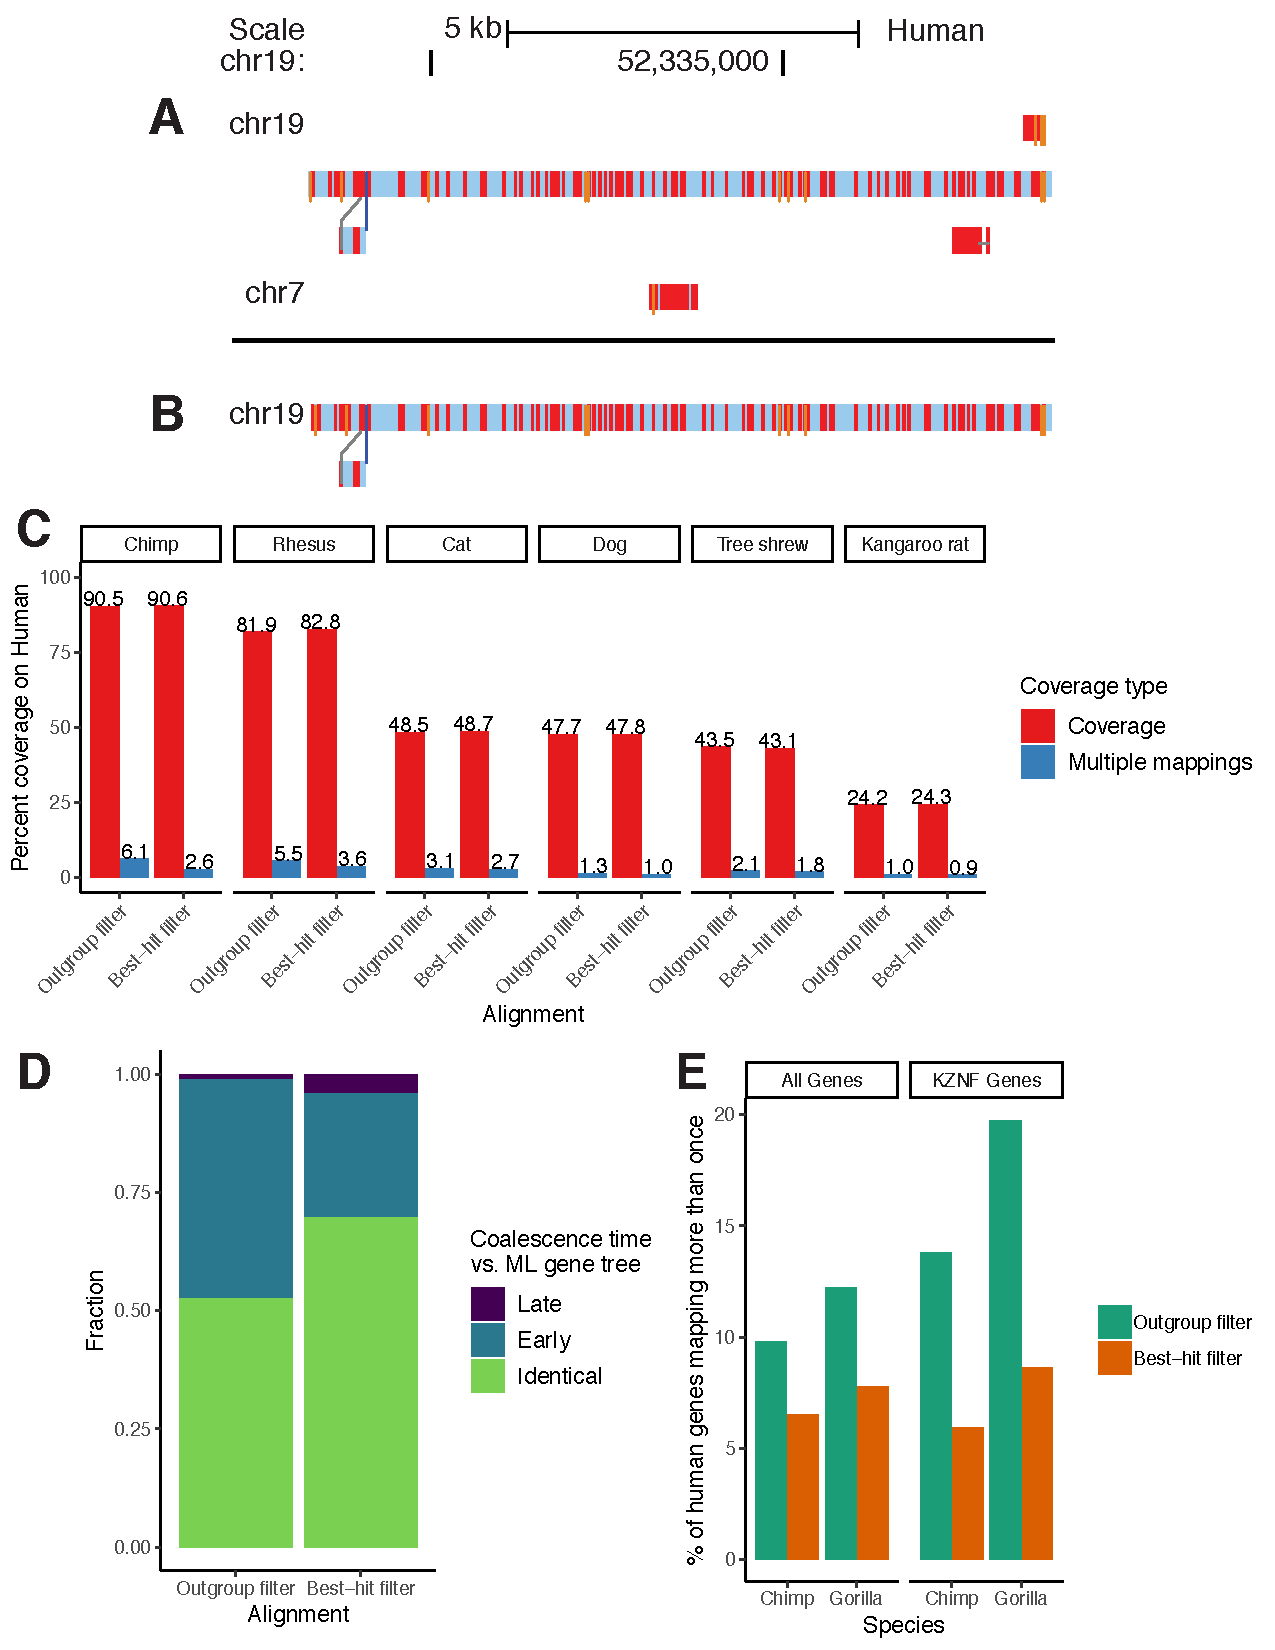
\includegraphics[width=\textwidth]{mapqfig.pdf}
\caption[Results from the improved paralog-filtering method]{Results from the improved paralog-filtering method. A/B: A sample snake track~\cite{assemblyHub} within a recently duplicated region before (A) and after (B) the filtering change. Nucleotide subsitutions are shown as red bars, and insertions are shown as thin orange bars. C: Coverage results from two alignments of identical assemblies using the outgroup and best-hit filtering methods. Multiple-mappings: sites which map to two or more sites on the target genome. D: Results from comparing phylogenetic trees implicit in the HAL alignment to ML re-estimated trees of the same regions. ``Early'' coalescences imply that too many duplication events have been created in the reconciled trees, while ``Late'' implies that too many loss events have been created. E: Percent of human genes that map more than once to the chimp/gorilla genomes in two CAT~\cite{cat} annotations using alignments created with the outgroup and best-hit filtering methods. KZNF: KRAB zinc-finger genes.}\label{fig:mapQ}
\end{center}
\end{figure}


\subsection{600-way amniote alignment}

\label{sec:600wayResults}
To demonstrate Progressive Cactus we present results from an alignment of 605 amniote genomes, relating in a reference-free manner a total of over 1 trillion bases of DNA across hundreds of millions of years of genome evolution. The amniote-wide alignment combines two smaller alignments: one created for the 200 Mammals project~\cite{200mPerspectivesPiece}, representing 242 placental mammals, and one for the Bird 10K project~\cite{b10kProjectAnnounce}, which relates 363 avians. The overall topology is shown in \figref{fig:600way}A. To our knowledge this represents the largest whole-genome alignment yet created. \tabref{tab:600wayStats} contains aggregate statistics on this alignment, which was computed using the Amazon Web Services (AWS) cloud infrastructure (for details on the construction, see \secref{sec:600waySupplement}).

Coverage within the 600-way alignment closely tracks phylogenetic distance and genome size, e.g.\ a median coverage on human of 2.3 Gb from Euarchonta species, vs. 1.2 Gb from Laurasiatheria species and 1.0 Gb from Glires species (\figref{fig:600way}B,C). The ancestral reconstructions within the 600-way alignment are highly complete, especially for functional sequence: 86\% of human coding bases are represented in our reconstruction of the ancestor of all placental mammals, while 95\% of chicken coding bases are represented in our reconstruction of the common ancestor of avians (\figref{fig:600way}D,E). Due to the long branch length ($\sim$0.7 substitutions-per-site divergence between the two clades), the amniote (human-chicken) ancestral assembly has a much lower proportion of reconstructed sequence than its immediate children, the avian and eutherian ancestors, e.g. retaining 16.3\% of chicken intron bases vs. 84.4\% in the avian ancestor, and 7.2\% of human intron bases vs. 56.5\% in the eutherian ancestor. However, coding bases are still well-retained (86.8\% from chicken and 58.7\% from human). The ancestral assemblies consistently contain a relatively higher proportion of sequence for avians than for mammals even across similar phylogenetic distance, reflecting a much more conservative mode of genome evolution in avians as well as the lower repeat content and denser gene content of avian genomes~\cite{zhang2014comparative}.

The ancestral reconstructions provide a history of substitution, indel, and rearrangement events. Though this history is by its nature only a hypothetical reconstruction of the true history of genome evolution along the tree, it is accurate enough to be useful. To demonstrate the utility of the indel history, we examined rates of small ($\le$ 20 bp) insertion and deletion events in the 600-way alignment. As expected given previous studies~\cite{indelRatesAcrossSpecies,crocs}, the rate of small indels in any given branch was correlated with the rate of nucleotide substitution (an $R^2$ of 0.69 for insertions and 0.80 for deletions in avians, and 0.39 and 0.40 respectively for eutherians), though the relative rates remained much lower for insertions (1.2\% of the substitution rate for both clades) and for deletions (2.4\% and 1.2\% of the substitution rate for avians and eutherians respectively). The corresponding fits are shown in \figref{fig:indelRatesAndRepeatStuff}A. Interestingly, we observe similar rates of deletions between eutherian and avian lineages, but evidence of a slightly increased rate of insertions in avians (\figref{fig:indelRatesAndRepeatStuff}(A)).
The ancestral assemblies also represent even difficult-to-align regions such as transposable elements. We ran RepeatMasker~\cite{repeatMasker} on several human ancestors, focusing on the recently-emerged L1PA6 family of L1 retrotransposons. When ascending the primate tree, approaching the origin of modern L1PA6 elements above the human-rhesus ancestor, L1PA6 elements appear increasingly similar to their consensus sequence (\figref{fig:indelRatesAndRepeatStuff}B).

Despite its scale, sub-alignments of the 600-way are similar to smaller alignments of the same species. Within the 7.1 billion aligned pairs involving human, mouse, rat, or dog within the 600-way, 76.49\% were present in an alignment less than a tenth the size (\figref{fig:cactusAlignmentComparisons}) --- this similarity is in line with that observed between different alignments of these same species\cite{earl2014alignathon}. As expected, the alignments more strongly agree in functional regions, such as coding exons, than for the genome as a whole (\figref{fig:regionSpecificJaccards}).
The size and fraction of functional elements reconstructed in ancestors shared between the 600-way and smaller alignments of mammals and, separately, avians was also highly similar (\figref{fig:mammalAncestorComparison}, \figref{fig:birdAncestorComparison}).
%% These effects are too small to worry about
%The amount of chicken sequence mappable to each ancestor is generally higher in the 600-way than in a smaller 48-bird alignment (\figref{fig:birdAncestorComparison}), while the amount of human sequence mappable to each of its ancestors is usually lower in the 600-way than in a smaller 11-mammal alignment (\figref{fig:mammalAncestorComparison}).
%Protein coding transcripts were mapped using protein-translated BLAT~\cite{BLAT}, and with the TranMap~\cite{transMap} projection alignment protocol with chained~\cite{kent2003evolution} human-chicken pairwise alignments from LASTZ~\cite{lastz} and 600-way alignment.

To evaluate the relative accuracy of the progressive alignment process back to the amniote ancestor, protein coding transcripts and genes were mapped using translated BLAT~\cite{BLAT}, translated BLAST~~\cite{BLASTPLUS}, LASTZ~\cite{lastz}, and the 600-way  (Section \ref{sec:transcriptMappingProtocol}).
Of 84,001 protein-coding human transcripts to chicken, BLAT mapped 70\%, BLAST mapped 80\%, LASTZ mapped 67\%, and Progressive Cactus mapped 74\%. Both Progressive Cactus and LASTZ had much lower levels of generally paralogous multi-mapping (2-3\% of transcripts) than either translated method (16\%-51\%) (Tables~ \ref{tab:humanChickenTranscriptMappingStats}, \ref{tab:humanChickenTranscriptAlignStats}, \ref{tab:humanChickenGeneAlignStats}).
% base 
Comparing Cactus and LASTZ coding sequence mappings to the union of the translated alignments, both in terms of individual gene counts and coding and mRNA bases, Cactus has a marginally higher fraction of shared elements with the translated alignments than LASTZ (\tabref{tab:humanGeneCdsToAlignedCmp}). 
Supporting this result, comparing the median per transcript and gene base-level Jaccard similarity of these mappings to chicken, Progressive Cactus and LASTZ were most similar, and Progressive Cactus was more similar to translated BLAT and Blast than LASTZ (Figures \ref{fig:transcriptCDSJaccards}, \ref{fig:geneCDSJaccards}; \tabref{tab:humanChickenTranscriptMappingMethodSim}). 
% existing annotation
Both Progressive Cactus and LASTZ have higher levels of base-level similarity with existing Chicken annotations than either translated alignment method (\tabref{tab:humanChickenTranscriptNativeSim}). 
%We note that In analyzing the distribution of gene mappings fractions is not uniform across transcripts, 69.2\% of chicken genes can map 50\% or more of their exonic bases to human, and 28.8\% are 95\% or more alignable to human (\figref{fig:chickenToHuman}).


%The base-level Jaccard similarity of these mappings to chicken between BLAT and BLAST is 0.57, LASTZ and Cactus is 0.78, while BLAT to LASTZ and Cactus is 0.59 and 0.64, respectively and BLAST to LASTZ and Cactus is 0.46 and 0.51 respectively. The LASTZ and Cactus projection methods produce fewer multi-mappings than BLAT or BLAST, which are presumed to be paralogous alignments.  The full results are shown in Tables~\ref{tab:humanChickenTranscriptMappingStats}, \ref{tab:humanChickenTranscriptMappingMethodSim},
%and %\ref{tab:humanChickenTranscriptAlignStats}.

The Bird 10K species were also separately aligned with MULTIZ~\cite{tba} using the chicken genome as the reference, allowing us to make a comparison between the two resulting alignments. Progressive Cactus aligned more total bases to chicken than MULTIZ (an average of 69.4\% of the chicken genome compared to an average of 64.9\%, for an average increase of 47 Mb). Since, unlike Progressive Cactus, MULTIZ is reference-biased, the difference is more stark when looking at the number of bases aligned to a genome not used as the MULTIZ reference (an average of 79\% of the zebra finch covered vs. 49.2\%, for an average increase of 367Mb: see \figref{fig:multizComparison}).

\begin{figure}
\begin{center}
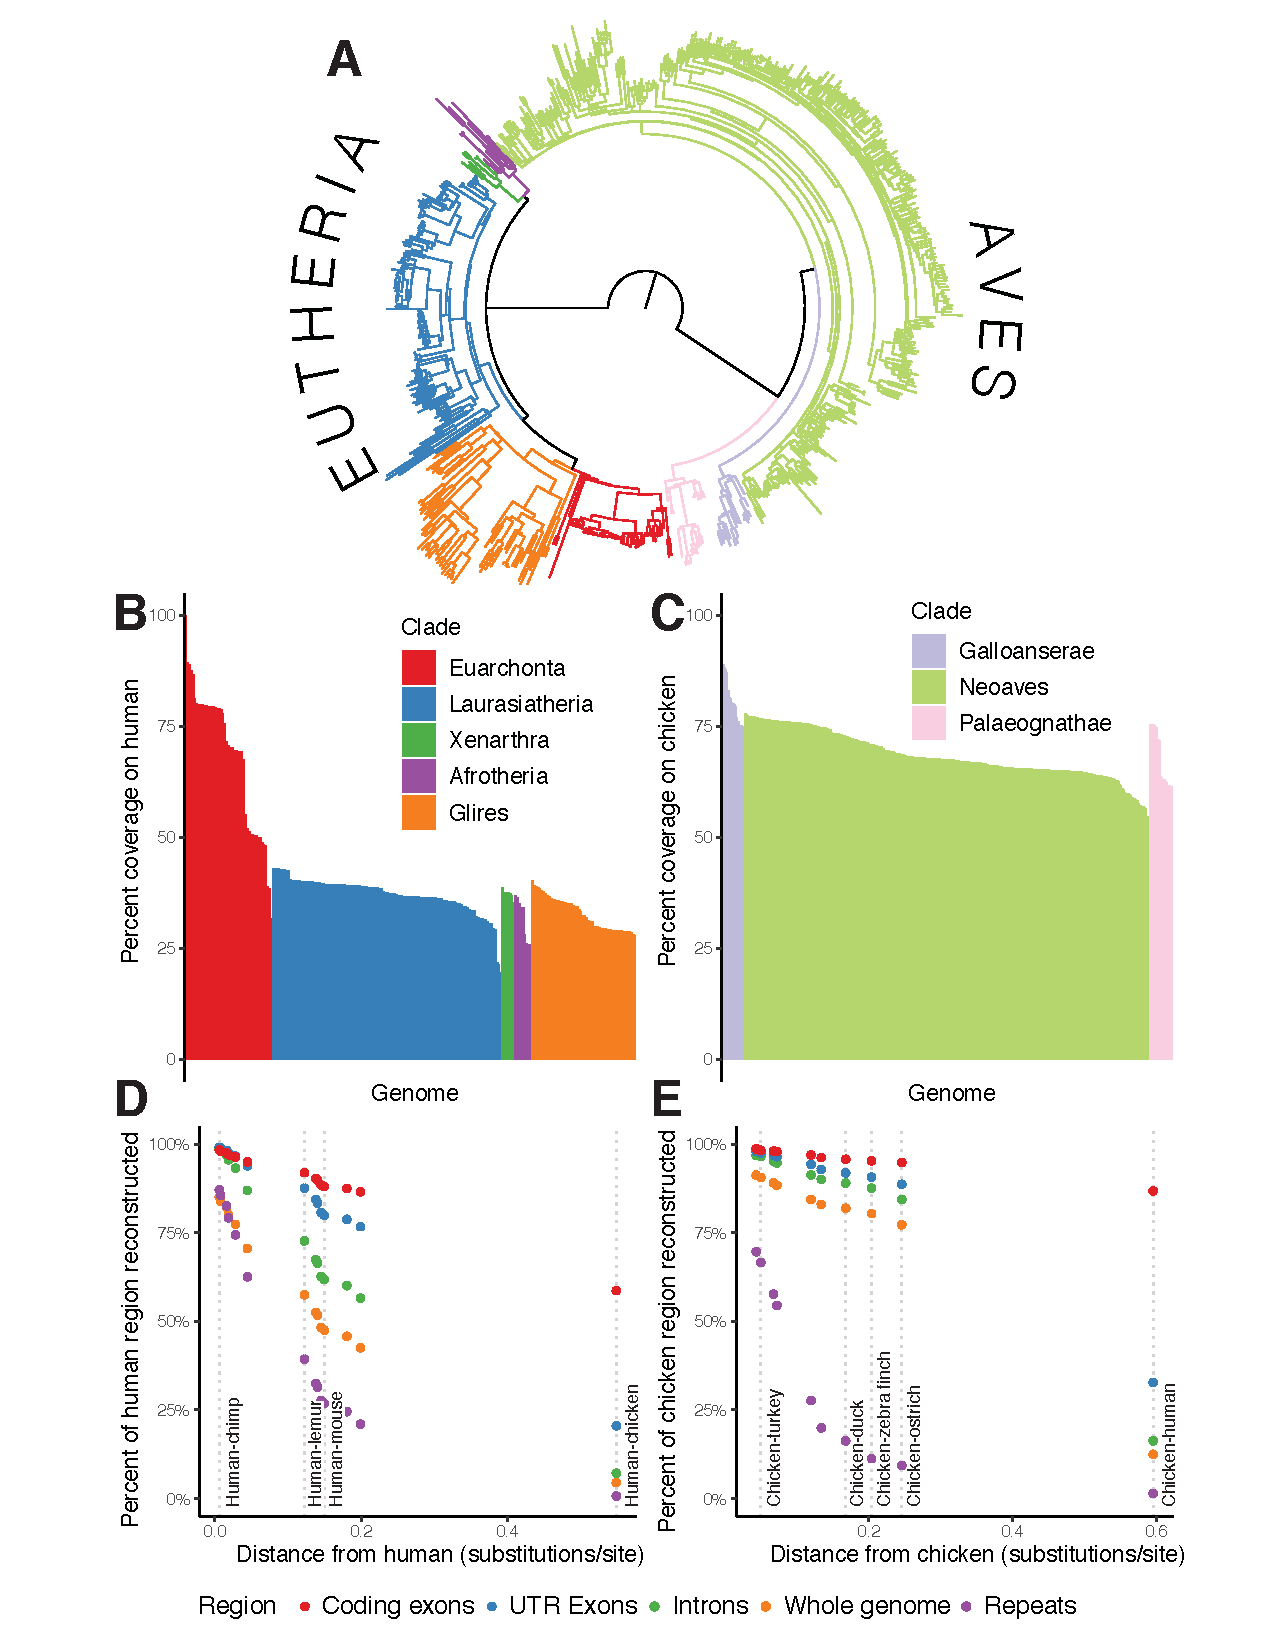
\includegraphics[width=\textwidth]{600wayfig.pdf}
\caption[Results from the 600-way amniote alignment]{Results from the 600-way amniote alignment. A: The species tree relating the 600 genomes. Branches are colored by clades in the same way as figures B and C. B: Percent coverage on human within the eutherian mammals, grouped by clade from highest to lowest coverage. C: Similar to B, but for coverage on chicken within the avian alignment. D: Percent of various regions within the human genome mappable to each ancestral genome reconstructed along the path leading from human to the root. The positions of selected ancestors are labeled by dotted lines to indicate useful taxonomic reference points as context. E: Similar to D, but for the path of reconstructed ancestors between chicken and the root. }\label{fig:600way}
\end{center}
\end{figure}

\begin{figure}
\begin{center}
\subfloat[]{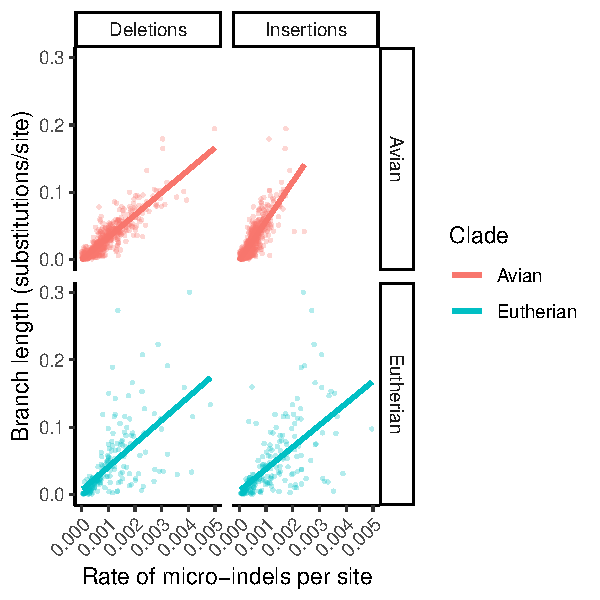
\includegraphics[width=0.5\textwidth]{indel_rates_breakdown_by_clade.pdf}}
\subfloat[]{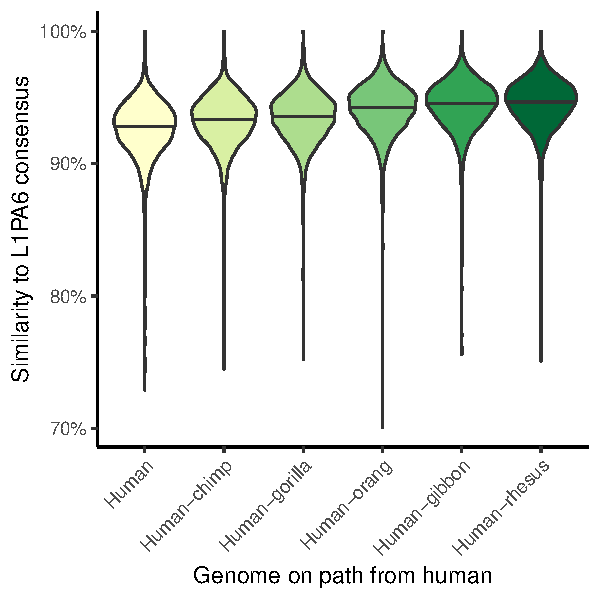
\includegraphics[width=0.5\textwidth]{rm_ancestor_divergence.pdf}}
\caption[Micro-indel rates and repeat reconstruction within the 600-way]{A: Rates of micro-insertions and -deletions (micro-indels) along each branch within the 600-way, compared to conventional substitutions/site branch length. The data from avian and eutherian branches are separated. Lines show a best-fit linear model for each category. B: Violin plot showing the increasing similarity to consensus of L1PA6 elements within reconstructed ancestral genomes along the path to the emergence of modern L1PA6 elements (in the human-rhesus ancestor). Horizontal lines indicate the median values.}\label{fig:indelRatesAndRepeatStuff}
\end{center}
\end{figure}

\begin{figure}
\begin{center}
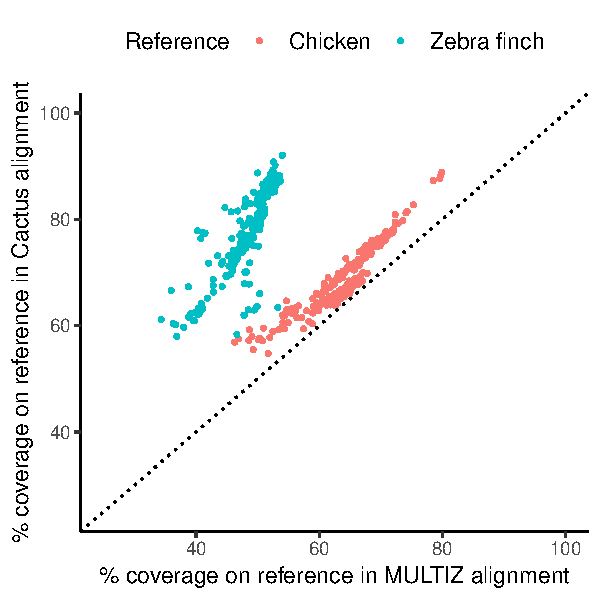
\includegraphics[width=0.5\textwidth]{multiz_vs_cactus_zebra_finch.pdf}
\caption[Coverage comparison between Progressive Cactus and MULTIZ avian alignments]{A comparison of coverage in the Progressive Cactus avian alignment compared to a chicken-referenced MULTIZ~\cite{tba} alignment of the same genomes. Coverage of both alignments on chicken and zebra finch is shown to illustrate the effects of reference-bias on the completeness of the MULTIZ alignment. Diagonal dotted line indicates a slope of 1 (i.e. if MULTIZ and Progressive Cactus coverage were equal).}\label{fig:multizComparison}
\end{center}
\end{figure}


\begin{table}
\begin{center}
\makebox[\linewidth]{
\begin{tabular}{l|r|l|r|l|l}
Alignment & \# of genomes & Total bases & Instance-hours & Core-hours & Common ancestor size \\
\hline
200 Mammals & 242 & 669 billion & 68,166 & 1.9 million & 1.73 Gb \\
Bird 10K & 363 & 400 billion & 5,302 & 0.2 million & 1.13 Gb \\
Combined & 605 & 1.07 trillion & 73,692 & 2.1 million & 181 Mb \\
\end{tabular}
}
\caption[Aggregate statistics for the 600-way alignment]{Aggregate statistics for the 600-way alignment. The increase in computational work for the mammal alignment over the bird alignment is largely caused by the increase in the pairwise alignment phase runtime, because it scales quadratically with the size of the genomes being aligned.}\label{tab:600wayStats}
\end{center}
\end{table}

\section{Discussion}
A few ambitious comparative genomics projects are already producing assemblies at the scale of tens to hundreds of species, and we anticipate that this scale of data will become much more common in the coming years. However, without a genome alignment it is impossible to relate these assemblies, and making an accurate genome alignment that large is difficult. We have demonstrated that Progressive Cactus can create alignments of hundreds of large genomes efficiently by producing an alignment relating over a trillion bases total. With this new development, we not only enable high-quality genome alignments for these projects, but also hope to set the stage for analysis of thousands to tens-of-thousands of genomes in the near future.

Furthermore, as long-read technologies become cheaper and more widely accessible, assembly quality has been rising. The age of having only a few high-quality vertebrate assemblies, like human or mouse, is at its end. As more assemblies converge on the gold-standard, ``reference'' level of quality displayed by GRCh38 and GRCm38, a reference-free genome alignment becomes increasingly useful. A reference-biased alignment forces the user to view genome evolution through the lens of a single, distant reference. As the average assembly becomes ever more complete and accurate, this missed opportunity to analyze regions not present in the reference grows worse. For this reason, we provide a reference-free alignment, allowing analysis of genome evolution throughout the entire tree rather than in comparison to one anointed reference.

Often a sequencing effort will produce multiple \emph{de novo} assemblies from different individuals, or diploid assemblies from a single individual. Progressive Cactus has already proved useful for comparison between assemblies of the same species~\cite{cat,greatApes,glennVGSV}.  Alignments of these assemblies are essential for many analyses, e.g.\ annotation of \emph{de novo} assemblies~\cite{cat}. Progressive Cactus should prove capable of capturing even complex structural variation, such as breakpoint resolved copy number variation, between these assemblies.

Producing a genome alignment has usually been an arcane task, where parameters used to produce, chain, or filter the input local alignments can have an under-appreciated effect on the result. We provide Progressive Cactus as an integrated pipeline that can be used across many different compute environments, but one that especially thrives on modern cloud environments. 
%% Omitting this as not described in methods:
%It intelligently adjusts alignment parameters to maximize efficiency and accuracy depending on evolutionary distance. 
While genome alignment is a computationally intensive task, we have broken up the problem into small pieces that can work in heterogeneous clusters, playing to the advantages of both cheap CPU-rich machines and more expensive memory-rich machines.

We have used Progressive Cactus to produce a 600-way alignment, which is, to our knowledge, the largest-yet genome alignment of vertebrates. This alignment is already proving useful for further downstream analysis. The Bird 10K~\cite{b10kProjectAnnounce} and 200 Mammals~\cite{200mPerspectivesPiece} consortia are using this alignment to analyze selection at unprecedented detail across avians and mammals, respectively.

% point out that the computational cost is mostly dependent on the
% local alignment phase and can be massively reduced by making that
% more efficient, especially for closely related genomes
%%I'm suggesting cutting this for brevity
%In the quest to make Progressive Cactus more efficient, optimizing the local alignment phase would offer the most return because the computational cost of the alignment is dominated by the generation of local alignments. Some less-sensitive local alignment programs are naturally more efficient than LASTZ, which is tuned for high sensitivity and long evolutionary distances. Making the local alignment phase a ``pluggable'' module, in which methods of generating the local alignments, or even the initial sequence graph, could be easily swapped out would be a fruitful avenue for experimentation. Progressive Cactus could potentially transition between using a less sensitive local aligner for closely related sequence and a more sensitive aligner across long evolutionary distance, much in the same way that we change alignment parameters based on evolutionary distance today.

As alignments become larger and more expensive to compute, it becomes much more important to be able to update them (by e.g.\ adding a new genome or updating an assembly) without recomputing the entire alignment. Progressive Cactus's framework, combined with special functionality in the HAL toolkit~\cite{hal} makes it possible to make these changes very efficiently: costing only a single subproblem's worth of computation time, usually about 120 CPU days. However, there is currently an appreciable amount of manual work involved in the process of adding, removing, or updating an assembly within an existing alignment. Making this simpler and more automated would be an interesting future direction, one that would potentially allow a very large alignment resource to be used and updated for years, with collaborators adding in their genomes of interest cost-effectively.


\section{Data availability}
The 600-way genome alignment is comprised of data gathered for the 200 Mammals project and data from the Bird 10,000 genomes (B10K) project. All the data is made available for immediate public use.

The 600-way alignment is available in HAL format at \url{https://alignment-output.s3.amazonaws. com/600way.hal}.

We also provide the subset of the alignment containing the 200 Mammals genomes at: \url{https://alignment-output.s3.amazonaws.com/200m-v1.hal}.

The subset of the alignment containing the Bird 10K genomes is at:
\url{https://alignment-output.s3. amazonaws.com/birds-final.hal}.

A visualization of the alignments and associated data is available by loading our assembly hub into the UCSC browser. By copying the hub link \url{https://comparative-genomics-hubs.s3-us-west-2.amazonaws.com/600way_hub.txt} into the "Track Hubs" page, the 605 genomes and associated tracks will be available.

%Note, the B10K consortium is organizing a phylogenomic paper and other analyses on the B10K data. We encourage you to contact us for collaboration if you are interested in using this data for phylogenetic analyses.

Note, the B10K consortium is organizing phylogenomic and other analyses with the avian alignment and sequencing data. We encourage persons to contact us for collaboration if they are interested in using this data for phylogenetic analyses.

\section{Code availability}
The Progressive Cactus pipeline is available at \url{https://github.com/ComparativeGenomicsToolkit/cactus} under the MIT license. The exact version of Progressive Cactus used for each of the analyses described above varies; the commit used in each analysis are available in the supplementary material.

\section{Acknowledgements}

Research reported in this publication was supported by the National Human Genome Research Institute of the National Institutes of Health under Award Numbers 1R01HG008742, R01HG009737, U54HG007990 and  2U41HG007234. Research reported in this publication was supported by the National Heart, Lung, And Blood Institute of the National Institutes of Health under Award Number U01HL137183. The content is solely the responsibility of the authors and does not necessarily represent the official views of the National Institutes of Health.

\section{Methods}

\subsection{Evaluation on simulated data}
\label{sec:simulationEvaluationSupplement}
20 primate genomes were simulated using Evolver~\cite{evolver}, managed using the evolverSimControl (\url{https://github.com/dentearl/evolverSimControl}, commit \texttt{\seqsplit{b3236deb}}) pipeline. The root genome used was derived from 30 megabases selected from the hg19 genome, and is available at \url{http://courtyard.gi.ucsc.edu/~jcarmstr/datastore/progressiveCactusEvolverSim.tar.gz} along with the Evolver configuration files that were used. The species tree used for the simulation was obtained from a catarrhine subtree of the 100-way alignment tree available on the UCSC browser. The tree used was, in Newick format:

\texttt{\seqsplit{(((((((Human:0.00655,Chimp:0.00684)anc0e:0.00122,Bonobo:0.00784)anc1e:0.003,Gorilla:0.008964)anc2e:0.009693,Orangutan:0.01894)anc3e:0.003471,Gibbon:0.02227)anc4e:0.01204,(((((Rhesus:0.004991,Crab\_eating\_macaque:0.005991)anc5e:0.001,Sooty\_mangabey:0.001)anc6e:0.005,Baboon:0.003042)anc7e:0.01061,(Green\_monkey:0.027,Drill:0.03)anc8e:0.002)anc9e:0.003,((Proboscis\_monkey:0.0007,Angolan\_colobus:0.0008)anc10e:0.005,(Golden\_snub-nosed\_monkey:0.0007,Black\_snub\_nosed\_monkey:0.0008)anc11e:0.004)anc12e:0.009)anc13e:0.02)anc14e:0.02183,(((Marmoset:0.03,Squirrel\_monkey:0.01035)anc15e:0.01065,White-faced\_sapajou:0.009)anc16e:0.01,Nancy\_Mas\_night\_monkey:0.01)anc17e:0.01)anc18e;}}

The alignments were generated using Progressive Cactus commit \texttt{\seqsplit{51eb980b}}. The input files (the simulated genomes as well as input files and Progressive Cactus configuration file) are available at \url{http://courtyard.gi.ucsc.edu/~jcarmstr/datastore/progressiveCactus.EvolverSim.CactusInput.EvenlySpread.tar.gz}. A non-default configuration (included in the dataset) was used to change the alignment filtering in both runs to better support the high degree of polytomy in the star-tree runs. Four sets of 2, 6, 10, and 20 genomes were used, each of which were run three times to generate runtime estimates. The sets are as follows:
\begin{itemize}
    \item 2 species:
    \begin{itemize}
        \item Rhesus
        \item Marmoset
    \end{itemize}
\item 6 species:
\begin{itemize}
    \item Species from 2-species alignment
    \item Gorilla
    \item Drill
    \item Black snub-nosed monkey
    \item White-faced sapajou
\end{itemize}
\item 10 species:
    \begin{itemize}
    \item Species from 6-species alignment
    \item Human
    \item Sooty mangabey
    \item Proboscis monkey
    \item Nancy Ma's night monkey
    \end{itemize}
\item 20 species:
    \begin{itemize}
        \item All species
    \end{itemize}
\end{itemize}
The runtime statistics were gathered using the \texttt{toil stats} command (the overall \texttt{Clock} time was used, which represents CPU time spent across all jobs). To generate the recall and precision statistics, MAFs were exported for each run (using \texttt{hal2maf} with the \texttt{-{}-onlyOrthologs} option using the rhesus genome as a reference) and compared to the Evolver MAF using mafComparator (\url{https://github.com/dentearl/mafTools}, commit \texttt{\seqsplit{82077ac3}}).
\subsection{Comparison using Alignathon data}
For comparison against other genome alignment methods, we aligned data (both the simulated "primates" and "mammals" datasets) used in the Alignathon~\cite{earl2014alignathon} using  Progressive Cactus. For comparison, we downloaded all the original Alignathon entries in MAF format. We used the original Alignathon analysis workflow (\url{https://github.com/dentearl/mwgAlignAnalysis}) to reanalyze the MAFs, with the output of the newest Progressive Cactus version added, to generate the precision / recall statistics (which we extracted from the comparison against the MRCA truth set). The simulated-mammal results are shown in \tabref{tab:alignathonMammals}, and the simulated-primates results are shown in \tabref{tab:alignathonPrimates}.

\subsection{Adding a new genome to the simulated alignment}

We evaluated the accuracy of adding a genome to an existing alignment by  creating a new alignment of 19 of the 20 simulated genomes described above (holding out the ``Crab\_eating\_macacque'' genome), then adding it back in after the fact. All alignments for this analysis were generated using Progressive Cactus commit \texttt{\seqsplit{49e80082}}.

To add the crab-eating macaque back in as the child of an existing node (the add-to-node strategy), we ran a single new alignment with the tree \texttt{(Rhesus:0.006, Crab\_eating\_macaque:0.007, Sooty\_mangabey:0.001)anc6e;}. The anc6e genome from the original, held-out alignment was used as a unreconstructed ancestral input sequence. We set the ``runMapQFiltering'' option in the config file to ``0'' and the ``alignmentFilter'' option to ``singleCopyOutgroup'', since these options produce a better alignment of polytomies. We merged the resulting HAL file into a new copy of the existing alignment via the command \texttt{\seqsplit{halReplaceGenome <copy of held-out alignment> anc6e -{}-topAlignmentFile <held-out alignment> -{}-bottomAlignmentFile <add-to-node alignment>}}.

To add the macaque by splitting a branch (the add-to-branch strategy), we ran two separate alignments. We ran the first with the tree \texttt{(((Rhesus:0.004991, Crab\_\allowbreak eating\_\allowbreak macaque:0.005991)\allowbreak anc5e:0.001, Sooty\_\allowbreak mangabey:0.001)\allowbreak anc6e:0.005, Baboon:0.003042)\allowbreak anc7e;} (with the \texttt{-{}-root anc5e} option so that only a single subproblem was run), generating a newly reconstruted anc5e ancestor. We then ran a second alignment with the tree \texttt{(anc5e:0.001, Sooty\_\allowbreak mangabey:0.001)\allowbreak anc6e;}, again providing the anc6e assembly from the original alignment rather than inferring a new reconstruction. (We note that these two subproblems could have been run in a single alignment invocation, resulting in the same amount of alignment work but a slightly more complicated merging process.) To merge these two add-to-branch intermediate alignments into a full alignment, we first removed the Rhesus genome from a new copy of the held-out alignment. We then ran \texttt{halAddToBranch <held-out alignment> <first add-to-branch alignment> <second add-to-branch alignment> anc6e anc5e Rhesus Crab\_\allowbreak eating\_\allowbreak macaque 0.001 0.006}.

We evaluated the performance of these new alignments using mafComparator in the same way as described in \secref{sec:simulationEvaluationSupplement}. In the interest of narrowly determining accuracy of alignments involving the newly added genome, we counted only aligned pairs involving the Crab\_eating\_macaque genome when calculating precision, recall, and F1 scores.

\subsection{Evaluation of the effect of the guide tree}
\label{sec:guideTreeSupplement}
The guide-tree analysis was performed on a set of 48 bird genomes originally published in 2014~\cite{jarvisSpeciesTree}. To reduce the amount of alignment work required, we subsetted these genomes down to the size of only a single chromosome, chicken chromosome 1 (by removing any contig or scaffold which had less than 20\% of its sequence alignable to chicken chromosome 1). We used Progressive Cactus commit \texttt{\seqsplit{36304707}} for all alignments in this analysis.

The Prum and Jarvis topologies were adapted from \cite{prumSpeciesTree} and \cite{jarvisSpeciesTree}, respectively. The ``permuted'' topology was generated starting from the Jarvis topology, via 3 randomly chosen subtree-prune-regraft operations followed by 3 random nearest-neighbor-interchange operations. Each of these three topologies had branch-length estimates performed using phyloFit from the PHAST package~\cite{phast} based on fourfold-degenerate sites of BUSCO orthologs. Finally, the ``Consensus'' tree was produced as a strict consensus of the Jarvis and Prum trees (collapsing all groupings that were not the same in both trees) using the \texttt{ape::consensus} method from the APE R package~\cite{apePackage}. The branch-lengths for this tree were generated from the fitted branch lengths for the two input trees, using the \texttt{consensus.edges} function of the phytools R package~\cite{phytoolsPackage}. The four final trees that were used in the four Progressive Cactus alignments are shown in \figref{fig:guideTreeTrees}, and available in supplementary data in Newick format.

We further focused on the alignments with guide trees based on Jarvis / Prum (\figref{fig:jarvisPrumCompare}) to establish what alignment differences resulted from different phylogenetic hypotheses. \figref{fig:jarvisPrumCompareMatrix} shows a refinement of the overall alignment-to-alignment F1 scores shown in \tabref{tab:f1scores}, showing the F1 scores for each species pair between the Jarvis- and Prum-based alignments. Each pair of species has an F1 score between Jarvis- and Prum-based alignments of at least 0.955.

\subsection{Impact of assembly quality on alignment quality}

We aligned two sets of 11 boreoeutherian genomes: one where 7 of the species were represented by relatively low-quality assemblies, and another where the same 7 species were represented by higher-quality assemblies, these are listed in \tabref{tab:assembly_quality_comparison_assemblies}. The remaining four genomes had the same assemblies in both alignments to facilitate comparison (human, hg38; mouse, mm10; rat, rn6; and dog, canFam3).

\subsection{Paralogy-filtering evaluation}
\subsubsection{Alignment of 12 Boreoeutherian genomes}
\label{sec:mapQAlignmentSupplement}
We ran two versions of Progressive Cactus (commits \texttt{\seqsplit{450da74}} [best-hit filtering] and \texttt{\seqsplit{aca859f}} [outgroup filtering]) using the following tree:

\texttt{\seqsplit{(((((Human:0.006969,Chimp:0.009727):0.025291,Rhesus:0.044568):0.07,Tree\_shrew:0.19):0.03,(Kangaroo\_rat:0.17,(Mouse:0.072818,Rat:0.081244):0.11):0.150342):0.02326,((Dog:0.07,Cat:0.07):0.087381,((Pig:0.06,Cow:0.06):0.104728,Horse:0.05):0.05):0.04);}}

The alignment files are accessible in the URLs listed at \tabref{tab:mapqHals}, and the assemblies used are listed in \tabref{tab:mapqAssemblies}. Coverage statistics from the resulting alignments were obtained using the \texttt{halCoverage} tool.

\subsubsection{Annotation using CAT}
\label{sec:mapQCATSupplement}
We produced two alignments using Progressive Cactus on the UCSC hg38, panTro6, and gorGor5 assemblies using the same Progressive Cactus versions mentioned above. We ran the CAT pipeline at commit \texttt{\seqsplit{7a8c7e24}}, using the GENCODE V30 gene set~\cite{gencode}. We projected the transcripts solely via transMap without the use of the AUGUSTUS modes. Multiple-mapping statistics as well as the gene composition of the final gene set were taken from the \texttt{filter\_tm\_metrics.json} file in the CAT output.

\subsubsection{Duplication-timing evaluation}
\label{sec:treeBuildingEvaluationSupplement}
The duplication-timing evaluation was performed using a custom pipeline (\url{https://github.com/joelarmstrong/treeBuildingEvaluation}) designed to sample columns from a HAL file and evaluate their trees against an independently re-estimated tree of the same region. For this analysis we used the the two  12-boreoeutherian alignments described above, sampling 10,000 columns from the human genome. The comparison trees were built from a context of 1000 bases around the entries in each sampled column using FastTree~\cite{fasttree} 2.1.10 and the \texttt{-gtr -nt} options. Only duplicated columns were counted in the final output (columns containing no duplications did not count in the results). The coalescence pairs were evaluated using the \texttt{-{}-onlySelf} option, meaning that only pairs that included the sampled site were counted in the results. To avoid weighting columns with a high number of copies per genome more than columns with a low number of copies per genome, only a single coalescence was randomly sampled per column.


\subsection{Generation of the 600-way alignment}
\label{sec:600waySupplement}
The 200 Mammals (200M) alignment was composed of two sets of genomes: newly assembled DISCOVAR assemblies and Genbank assemblies. The DISCOVAR genomes were masked with RepeatMasker~\cite{repeatMasker} commit \texttt{\seqsplit{2d947604}}, using Repbase~\cite{repbase} version 20170127 as the repeat library and CrossMatch as the alignment engine. The pipeline used is available at \url{https://github.com/joelarmstrong/repeatMaskerPipeline}. The guide-tree topology was taken from the TimeTree database~\cite{timetree}, and the branch lengths were estimated using the least-squares-fit mode of PHYLIP~\cite{phylip}. The distance matrix used was largely based on distances from the 4d site trees from the UCSC browser~\cite{ucscBrowser}. To add those species not present in the UCSC tree, approximate distances estimated by Mash~\cite{mash} to the closest UCSC species were added to the distance between the two closest UCSC species. The final guide tree is embedded in the HAL file, and available using the \texttt{halStats -{}-tree} command.

The 363 assemblies in the B10K alignment comprised four sets: 236 newly sequenced species for the ``family'' phase of the project, assembled using SOAPdenovo2 and AllpathsLG, 42 assemblies already sequenced from the ``order'' phase of the project, 36 assemblies taken from GenBank, and 49 assemblies contributed by other research groups. For the avian guide-tree, we used a tree that the B10K consortium derived as preliminary data from ultraconserved elements.

Both alignments were run on the AWS cloud over the course of 3 weeks for the avians and 2 months for the mammals, using a maximum of 240 \texttt{c3.8xlarge} instances and 20 \texttt{r3.8xlarge} instances. Because Toil's autoscaling mode was used, this capacity was only fully utilized during the initial phase of the alignment, when the potential for parallelism was at its highest.

The 600-way alignment was formed by aligning the two roots of the B10K and 200M alignments, using the xenTro9 (frog), latCha1 (coelacanth), and danRer11 (zebrafish) assemblies as outgroups. This created a ``linker'' alignment connecting the roots of the two alignments. The B10K and 200M alignments were then added to this linker alignment using the \texttt{halAppendSubtree} command.

\subsection{Micro-indel events within the 600-way}
We extracted all insertion and deletion events by running the \texttt{halBranchMutations} tool on every branch in the 600-way alignment. The ungapped insertion and deletion calls (represented by ``I'' and ``D'' respectively within the output file) were filtered so that only calls spanning less than 20bp (in the child for insertions, and the parent for deletions) were counted. The rate for each branch was then obtained by dividing the count of these micro-indel events by the total amount of sequence present in the child.

\subsection{Repetitive elements within ancestral sequences}
We ran RepeatMasker~\cite{repeatMasker} on all ancestral assemblies of human within the 600-way alignment (using RepBase~\cite{repbase} version 20170127, selecting the ``primate'' repeat library and choosing CrossMatch as the alignment engine). We additionally ran the same pipeline against human (as existing annotations used the ``Homo\_sapiens'' repeat library). All ancestors up to human-rhesus had over 78\% of the human complement of L1PA6 elements (\figref{fig:rmAncestorCount}).

\subsection{Human/chicken transcript alignment protocols}\label{sec:transcriptMappingProtocol}
Protein-coding transcript annotations were obtained from the UCSC Genome browser
\cite{ucscBrowser} tables.  Human annotations are GENCODE V34 on hg38
(GRCh38/GCA\_000001405.27) and chicken annotations are Ensembl 85 on galGal4
(GCA\_000002315.2).  Predicted RNA sequences for each protein-coding transcript are extracted
from the genome.  Only gene annotations on the primary assemblies were used,
those on alternate loci, patches, and assembled sequences were dropped.
This results in 84,001 transcripts in 19,695 genes for human and
15,328 transcript in 14,499 genes for chicken. 
The human transcripts were then mapped from the human genome to the chicken genome.

The steps for each method are outlined below, although the actual execution was
done by partitioning the data and using a cluster. Command-line tools from the
UCSC Genome Browser group are used for processing the resulting alignments.

\subsubsection{BLATX transcript alignment protocol}
The \textit{BLATX} alignments were created using protein-translated
mode to align the mRNAs to the target genome with \textit{BLAT}~\cite{BLAT}
version 36x5.  They were then filtered following the same protocol the UCSC
Genome Browser uses for creating the other species RefSeq alignments:

\begin{verbatim}
    blat -noHead -q=rnax -t=dnax -mask=lower <dest-genome.2bit> \
        <src-rna.fa> <dest-rna-raw.psl>
\end{verbatim}

We then filter to get near-best in genome.  Alignment to chicken uses near best filter
of \code{-localNearBest=0.010} while to human it uses \code{-globalNearBest=0.010}:

\begin{verbatim}
    faPolyASizes <src-rna.fa> <src-rna.polya>
    pslCDnaFilter <nearBestOption> -minId=0.35 -minCover=0.15 -minQSize=20 \
        -ignoreIntrons -repsAsMatch -ignoreNs -bestOverlap \
        -polyASizes=<src-rna.polya> <dest-rna-raw.psl> <dest-rna-mapped.psl>
\end{verbatim}

The \code{transMapPslToGenePred} command is then used to project the original CDS
onto the alignment.

\subsubsection{TBLASTX transcript alignment protocol}
The \textit{TBLASTX} alignments were created using protein-translated
\textit{tblastx} program to align the mRNAs to the target genome with
\textit{BLAST+}~\cite{BLASTPLUS} version 2.10.0+.

The database is created using the repeat masking from the UCSC Genome Browser
genomes to match what is used with in the \textit{BLATX} methodology above:
\begin{verbatim}
    convert2blastmask -in <dest-genome.fa> -masking_algorithm repeat \
        -masking_options "repeatmasker, default" -outfmt maskinfo_asn1_bin \
        -out <dest-genome.mask>
    makeblastdb -dbtype nucl -in <dest-genome.fa> -mask_data <dest-genome.mask>
\end{verbatim}

The mRNAs are aligned and the resulting XML converted to PSL format, filtering to an
e-value threshold of 0.01.  These are then chained using a program the UCSC group
developed for chaining \textit{BLAST} alignments:
\begin{verbatim}
    tblastx -db <dest-genome.fa> -db_soft_mask 40 -outfmt 5 -query <src-rna.fa> \
        -out <dest-rna-raw.xml>
    blastXmlToPsl -eVal=0.01 <dest-rna-raw.xml> <dest-rna-raw.psl>
    simpleChain -outPsl -maxGap=75000 <dest-rna-raw.psl> <dest-rna-chained.psl>
\end{verbatim}

The alignments produced are then filtered in the same manner as the \textit{BLATX}
alignments.


\subsubsection{LASTZ transcript alignment protocol}
Both the \textit{LASTZ}~\cite{lastz} and \textit{Cactus} transcript mappings uses the
\textit{TransMap}~\cite{transMap} projection alignment algorithm to project
transcript annotation between genomes.

The \textit{LASTZ} alignment chains and nets
\cite{CHIAROMONTE_2001,lastz,kent2003evolution,Schwartz_2003} were obtained from the
UCSC Genome Browser downloads.  These were then filtered to produce a set of
syntenic mapping chains using these steps:

\begin{verbatim}
    netFilter -syn <genomes.net> <syntenic.net>
    netChainSubset -wholeChains <syntenic.net> <genome.chain> <mapping.chain>
\end{verbatim}

\subsubsection{Cactus transcript alignment protocol}
The \textit{Cactus} alignments are extracted for all primary chromosomes from the HAL
file and chained using the same chaining algorithm as the \textit{LASTZ} chains, with
the \code{--noDupes} option having a similar effect as the syntenic net filtering:
\begin{verbatim}
   halLiftover --outPSL --noDupes 600way.hal <srcOrganism> \
      <srcChroms.bed> <destOrganism>  <src-dest.psl> <genome.psl>
   axtChain -psl -linearGap=loose -scoreScheme=HoxD55.q <genome.psl> <mapping.chain>
\end{verbatim}

The \textit{TransMap} protocol is use for both the \textit{LASTZ} and
\textit{Cactus} mapping chains to produce alignments of the transcripts to the
other genomes.  This used the \textit{pslMap} command to do the mapping and
\textit{pslRecalcMatch} to update the statistic in the alignments:

\begin{verbatim}
    pslMap -chainMapFile <src-rna.psl> <mapping.chains> <dest-rna-over.psl>
    pslRecalcMatch <dest-rna-over.psl> <dest-genome.2bit> <src-rna.fa> <dest-rna-raw.psl>
\end{verbatim}

The alignments produced are then filtered in the same manner as the \textit{LASTZ}
alignments.

\subsubsection{Transcript and gene alignment subsets and comparison}
To facilitate the comparative analysis of the alignment methods, we have created
reduced sets of the alignments using two different approaches.

While both \textit{BLATX} and \textit{TBLASTX} will align UTR, the strength of
protein-translated methods is in recognizing distant coding sequence relationships.  We have
previously shown \cite{transMap} alignment projection-mapping methods align more UTR
bases than translated methods.  To facilitate comparisons, CDS alignments from each method were
created by trimming the RNA alignments to contain only the CDS regions as defined by the human annotation set.

While mapping all transcripts is useful, particularly for understanding the utility of the methods
in assisting genome annotation, individual transcripts overlap, biasing assessment of transcribed mappings to genes 
with larger transcript numbers. To remove most of this base multiplicity from comparisons, in addition to showing full transcript results, subsets of the
alignments are creating using only one representative transcript per gene.
For the full RNA alignments, the longest RNA for each gene was chosen, with
the CDS alignments choosing the transcript with the longest CDS.  The
biology of overlapping gene structures and the ambiguities in defining genes cause
around $4\%$ of genomic bases to appear in more than one gene in the RNA and $3\%$ in the CDS gene sets due to overlap.

Individual pairwise alignments were compared at the base-level, consistent with the earlier comparisons reported.  Briefly,
alignment similarity is computed by comparing the set of shared aligned pairs. That is, a pairwise alignment can be viewed as a set of aligned base pairs, each a coordinate from the source (human) and target (chicken) genome. The Jaccard index is, in this context, the number of aligned pairs identical between the two alignments divided by the union of all aligned pairs in the two alignments. It is worth noting that translated alignments are encoded for comparison using their induced base-level alignments.
 Transcripts or genes that aren't aligned by either of the aligners being compared are assigned Jaccard indexes of zero.
 
To account for human bases which map to multiple bases in chicken (which occurs frequently for the translated alignment methods that include very distant, fragmented, paralogous alignments, but much less often for the non-translated methods), 
  when comparing the alignments of an mRNA or CDS between two methods, if either or both methods produces multiple alignments, we pick the pair of mappings (one from each method) with highest shared similarity to report. This generally has the effect of removing distant paralogies from the comparison. 

%to see how the alignments methods
%handle a diversity of transcripts and their utility in genome annotation, they
%also have a bias in that the projection methods use the same genomic alignment
%regions to map overlapping transcripts, with translated methods aligning each
%transcript independently.  

%\subsubsection{Comparison of alignments}\label{sec:jaccardCalculation}

%Comparisons of alignments are done using the Jaccard index\cite{jaccard_index}
%(similarity coefficient).  The similarity is computed using the base
%similarity of the two alignments on the given genome.  Transcripts that aren't aligned by either of the aligners being compared are assigned Jaccard indexes of zero.  When summarizing
%similarities, the mean rather than the median is used as the median has a bias against
%methods that produce paralogous alignments, which results in large numbers of
%zero Jaccard indexes.

\subsection{Progressive Cactus Methods}

Progressive Cactus builds upon the original Cactus program, in particular the CAF and BAR algorithms, which are described in detail in the original publication \cite{cactusGenomeRes}. In overview, the CAF algorithm (short for Cactus Alignment Filter) is an algorithm designed to construct a sequence graph from an input set of local alignments (in Progressive Cactus computed using LASTZ\cite{lastz}). We omit a complete definition here, but a sequence graph represents the alignment of a set of nucleotide strings. It can formally be represented using a bidirected or biedged graph~\cite{pmid15342561, pmid19645596, pmid29461862} (\figref{fig:cactus_explanation_fig}(A)). Larger nucleotide strings are encoded as  walks through sequence graphs (\figref{fig:cactus_explanation_fig}(B)); in the biedged representation an alignment between two or more substrings is represented by both strings visiting a common sequence edge; in Progressive Cactus each sequence edge represents an alignment `block', a set of oriented substrings in the set of input strings which are considered to be gaplessly aligned. A key property of alignments represented by sequence graphs is that the alignments they represent are equivalence relations: that is alignments are transitive, reflexive and symmetric. The core challenge the CAF algorithm addresses is sub-selecting which local alignments from the input set to include in the sequence graph, because typically a collection of local alignments computed with a tool like LASTZ will contain numerous transitive inconsistencies which when combined will create implausible, high-degree alignment blocks in the sequence graph. The CAF algorithm uses the 3-edge connected components of a sequence graph to define a restricted from of cactus graph such that there exists a homomorphism from the alignments blocks in the sequence graph onto the resulting cactus graph (\figref{fig:cactus_explanation_fig}(C)). In the constructed cactus graph each edge is a member of exactly one simple cycle. These simple cycles correspond to `chains' of alignment blocks, maximal sequences of blocks whose aligned substrings appear in the same order and orientation in the input strings. The CAF algorithm iteratively filters the input set of alignments to remove local alignments that create short simple cycles in the cactus graph, this is achieved by deleting alignments blocks from the sequence graph involved with these short cycles. The result of the CAF algorithm is a filtered set of local alignments represented using a sequence graph. To add to the output sequence graph of the CAF algorithm the BAR algorithm constructs a detailed alignment by extending gapped alignments from the ends of each alignment block, using a greedy approach to force consistency between the alignments constructed starting from connected alignment blocks. In Progressive Cactus the CAF and BAR algorithms are applied to create an alignment for each internal of a guide tree of the corresponding set of in-group and out-group species.

Below we provide updates on the changes made to Cactus to create Progressive Cactus.

\begin{figure}
\begin{center}
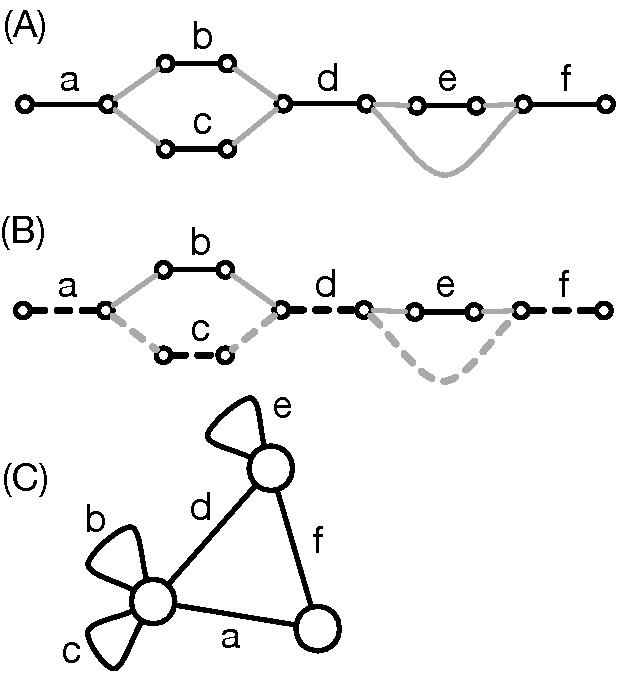
\includegraphics[width=5cm]{cactus_explanation_fig.pdf}
\caption[]{Sequence and cactus graph example. (A) A biedged sequence graph constructed from the strings `a b d e f', `a c d e f' and `a b d f', where here homology is indicated by common alphabet characters. In Progressive Cactus the sequence edges (black lines) represent alignment blocks. The adjacency edges (grey lines) indicate the sequence relationships. (B) Each input string is encoded as a restricted form of walk in the sequence graph; the path for the string `a c d f' is highlighted by dotted edges. (c) The cactus graph constructed from the sequence graph using the Cactus construction procedure (see \cite{cactusJCompBio} for details). The subsequence `a d f' common to all the input strings is represented by a simple cycle, termed a chain. The remaining substrings `b', `c', and `e' are each in trivial chains represented using self loops.}\label{fig:cactus_explanation_fig}
\end{center}
\end{figure}

\label{sec:cactusMethods}
% Moved from supplementary materials
\subsubsection{Preliminary repeat-masking}
% v have done this, hopefully
%\todo{This needs a pointer to the code, and the command line flags we use for lastz - is to vague as it stands}
Progressive Cactus requires input genomes to be soft-masked, but often repetitive sequence goes unmasked due to poor masking or incomplete repeat libraries for newly-sequenced species. This can negatively affect alignment runtimes (as alignments need to be enumerated to and from all copies of a repetitive sequence) and impact quality. For this reason, we mask overabundant sequence before alignment, using a strategy not based on alignment to repeat consensus libraries, but on over-representation of alignments. We first divide each genome into small, mutually overlapping chunks. For each chunk, we align it to itself and a configurable amount of other randomly sampled chunks (currently 20\% of the total pool). To avoid combinatorial explosion due to unmasked repetitive sequence, we use a special mode of LASTZ~\cite{lastz} which stops exploring alignments from any region early if a maximum depth is reached (using the flag \texttt{-{}-queryhsplimit=keep,nowarn:1500} which stops after an high-scoring-pair depth of 1500). We then soft-mask any region covered by more than a configurable number of these alignments (currently set to 50). Further details can be found in the \text{src/cactus/preprocessor} section of the Progressive Cactus codebase. Though the preprocessing step is automatically run as part of the pipeline, we also provide a \texttt{cactus\_preprocessor} utility to run only the preprocessor without producing a full genome alignment.
\subsubsection{Local alignment and outgroup selection}
The alignment process for each subproblem begins with a series of local alignments generated using LASTZ~\cite{lastz}. The local alignments fall into two sets: a set of all-against-all alignments among the ingroup genomes, and a set of alignments from ingroup genomes to outgroup genomes.

We have found outgroup selection to be absolutely crucial in creating an acceptable ancestral reconstruction: any missing data or misassembly in the outgroup that causes a true deletion in one of the ingroups to be misinterpreted as an insertion in others will mean that the ancestor contains less sequence than it ought to. This missing sequence in turn impacts the alignment between the entire subtree below the reconstructed ancestor and the entire supertree above it: the missing sequence will never be aligned between the subtree and supertree. To avoid this we attempt to use multiple outgroup genomes in each subproblem (3 by default). Naively aligning each ingroup against multiple outgroups would significantly increase the computation time; to avoid this we note that in general any region already containing an outgroup alignment benefits very little from aligning an additional outgroup. Therefore, we iteratively align each ingroup against one outgroup at a time, pruning away any ingroup sequence already covered by the previous outgroup alignments. In this way the computational cost is reduced to be far less than naively aligning against the entire outgroup set, while still retaining nearly all of the benefit. In addition, we allow the user to designate certain genomes in the input as being of particularly high quality; these are chosen as outgroups if possible to avoid problems with missing data in regions like mitochondrial or sex chromosomes that are often missing from some assemblies but not others.

\subsubsection{Paralogy resolution}
\label{sec:mapQ}

%\todo{Joel, please read this through}
% Read through it. Looks good (thanks for the addl figure). I made some minor edits to clarify things (in my view), feel free to revert if you prefer

In constructing the initial sequence graph during the CAF algorithm Progressive Cactus greedily chooses which pairwise alignments to include in an effort to prevent paralogous alignments between the ingroup species. We developed two algorithms. Both are greedy algorithms designed to rank the pairwise local alignments and then iteratively add the alignments to the graph, at each step choosing to accept or reject the addition of alignments to the graph. Each added alignment `glues' together two alignment blocks, splitting existing alignment blocks as necessary and merging the resulting two alignment blocks into one new block in the graph (\figref{fig:cactus_glueing_fig}). 

% Heuristics. Single-copy outgroup. MapQ and the basic logic behind it.
The first algorithm, which was used in previous, beta versions of Progressive Cactus, relied on an outgroup-based heuristic to resolve duplication timing. This heuristic, which we term ``single-copy outgroup filtering'', first sorts all the LASTZ alignments by their score in descending order. Then, starting from the highest scoring alignment, it iteratively adds one alignment at a time to the sequence graph, rejecting the glueing of any two blocks if the resulting alignment block would contain two or more substrings from the same outgroup genome. In this way the heuristic refuses to glue blocks when the resulting block would contain homologies that imply duplications in the outgroups. These self-homologies within the outgroup would necessarily involve duplication events that occurred above or outside of the subtree rooted at the MRCA of the ingroup genomes. Since the goal at each progressive step is to determine (the transitive closure of) orthology relationships within this subtree, refusing these outgroup self-homologies proves useful for assigning orthology between ingroups. Unfortunately, this method is very sensitive to incomplete outgroup assemblies (containing an incorrect number of copies of a duplicated region) or variation in similarity between closely related paralogs, causing assignment to the wrong copy. As seen in \figref{fig:mapQ}, this filtering method tended to resolve duplications far too early, often causing paralogs to be called as orthologs (for example, implicitly labeling 6.1\% of human sequence as duplicated along the chimpanzee lineage, which is certainly an overestimate).

To remedy this problem, we developed an improved duplication-timing method, which we termed ``best-hit filtering'' in the earlier text. The method preprocesses the local alignments to define for every base in every input genome a ranking by score of the local alignments that overlap it. The sequence graph is then built by first including the highest scoring alignment for each base in each genome. We refer to this highest-scoring set as the set of `primary' alignments and the remaining alignments the `secondary' alignments. Note this definition is asymmetric: a pairwise alignment may be primary for one of the substrings it aligns and secondary for the other. All primary alignments are added to the initial graph unconditionally because they represent the most likely ortholog relationship (or in the case of multiple orthology, likely a random ortholog) (\figref{fig:mapQMethodSupp}). The set of primary alignments represents a conservative set of alignment relationships that should include nearly no alignments to ancient paralogs. However, in regions that have undergone many rounds of lineage-specific duplications (which should all be aligned together in the restricted duplication-timing problem we describe above), the set of primary alignments will often by chance not align all copies together.
For this reason, after adding the primary alignments we iteratively add secondary alignments, going in descending order of score, rejecting any secondary alignment that would glue together any two existing blocks that both contain sequences from the same outgroup species (similarly to the ``single-copy outgroup filtering'' method) --- this allows lineage-specific duplications of ingroup genomes to correctly land in the same block, while avoiding merging blocks from likely-paralogous alignments.

\begin{figure}
\begin{center}
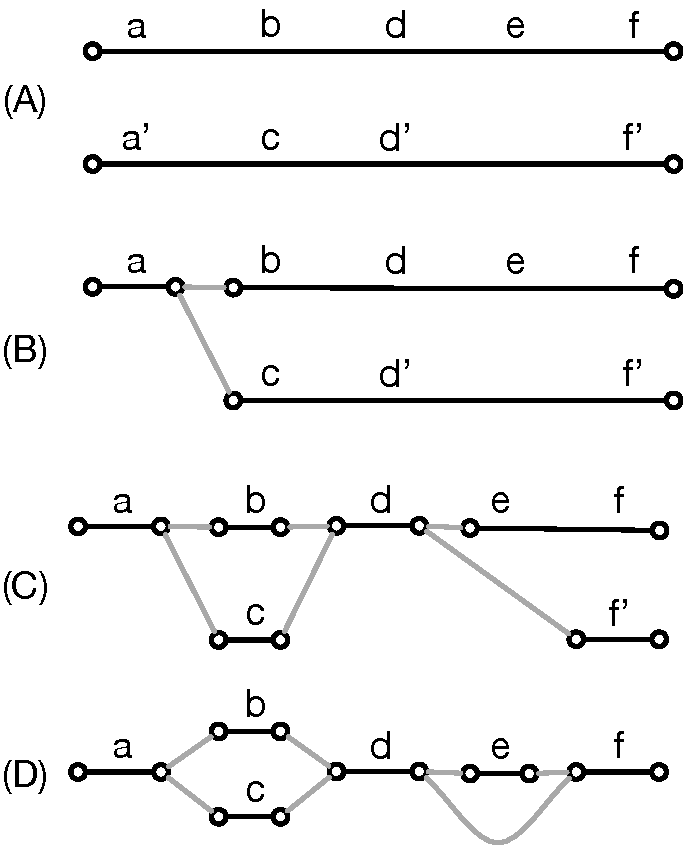
\includegraphics[width=5cm]{cactus_glueing_fig.pdf}
\caption[]{Iteratively building a sequence graph by progressive glueing operations. (A) Two sequence edges labeled with their respective strings. (B) A local alignment glues together the `a' copies. (C) The glueing of `d'. (D) The glueing of `f' creates the final set of alignment blocks. }\label{fig:cactus_glueing_fig}
\end{center}
\end{figure}

\begin{figure}
\begin{center}
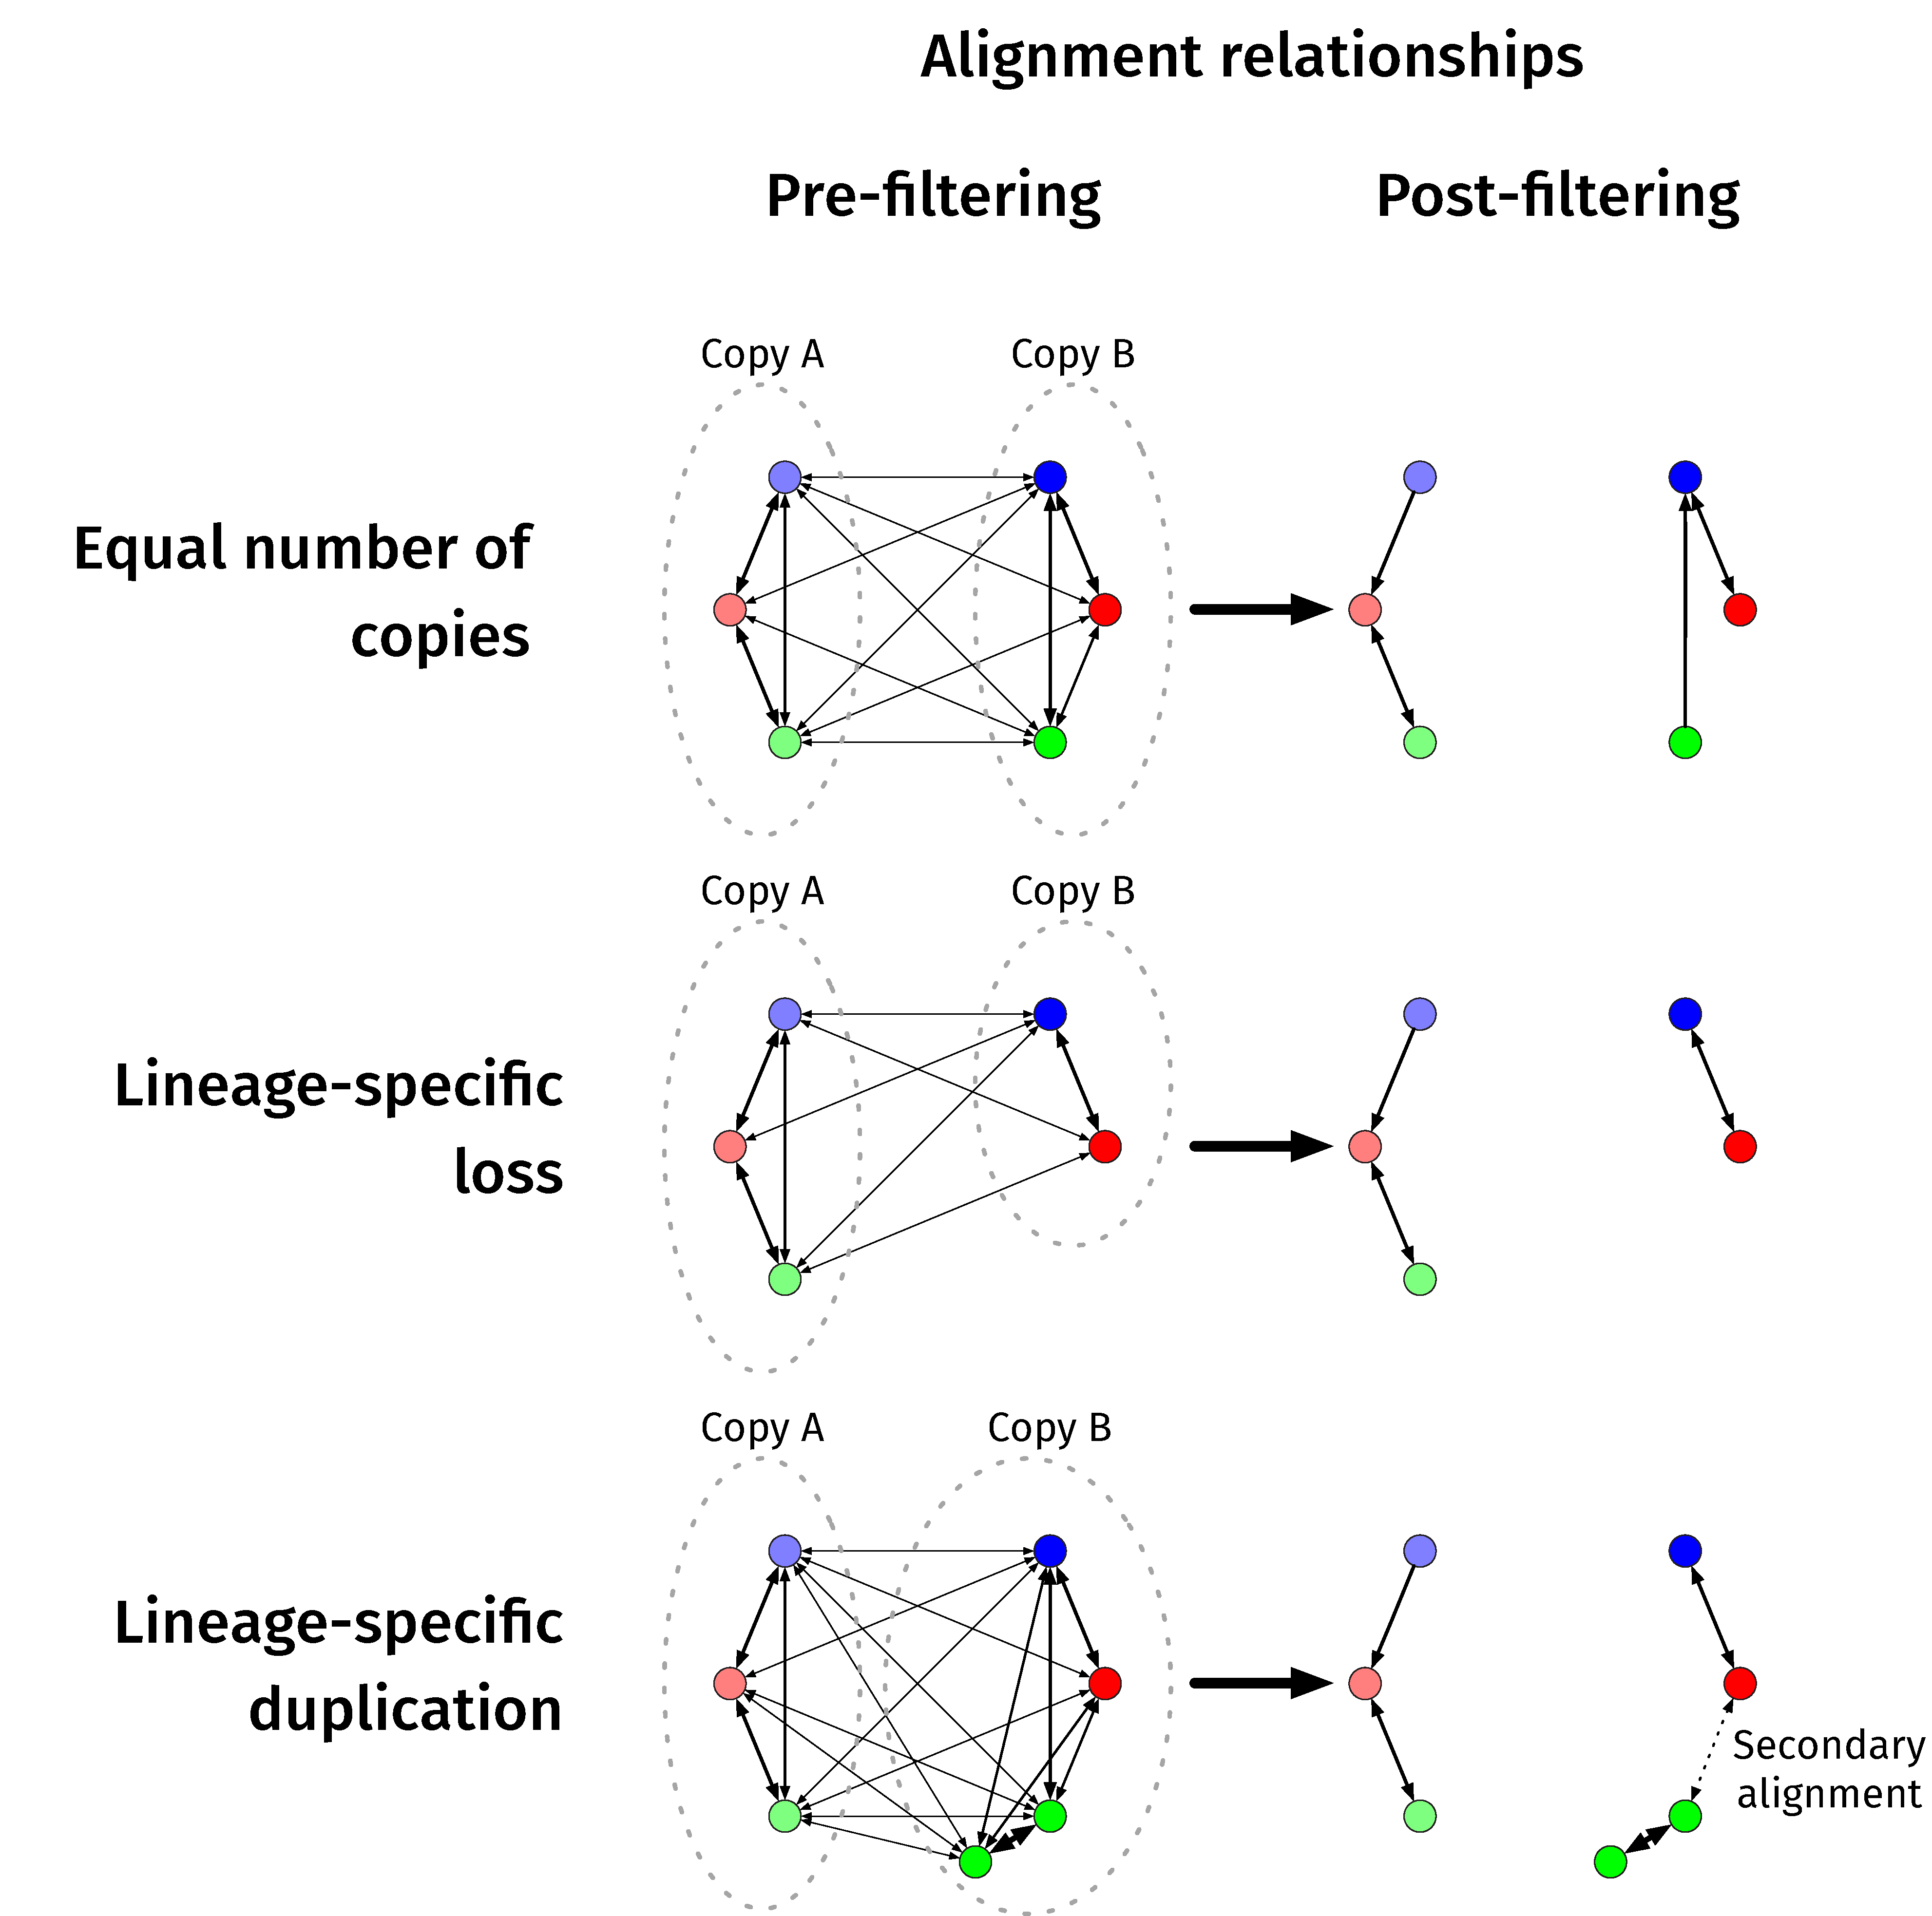
\includegraphics[width=\textwidth]{mapQfigure.pdf}
\caption{A visualization of the best-hit filtering method. Here, each node of the directed graph indicates a single base, and edges represent pairwise alignment relationships (the color of the node indicates the species the base belongs to, and higher thickness of edges represents higher scores of the pairwise alignments). Since Progressive Cactus's alignment columns represent the transitive closure of the input pairwise alignment relationships, the final alignment relationships will be represented by connected components within this graph. Taking the single best hit (so that this graph contains at most one outgoing edge per base) results in the correct separation between copies if orthologous copies have higher score, but some lineage-specific duplications require secondary, non-best-hit alignments to bring together orthologs from different species.}\label{fig:mapQMethodSupp}
\end{center}
\end{figure}


\subsubsection{Removing recoverable chains}
\label{sec:removeRecoverableChains}
\label{sec:recoverability}
%Due to the insensitive and approximate nature of the input local alignments, homologies are often missed in the input to the CAF algorithm. Alignment blocks that are ``incomplete'', i.e.\ contain some true homologies but miss others, can cause issues for the CAF algorithm: if these incomplete blocks make it into the output Cactus graph, the missing homologies can never be recovered by the BAR algorithm because to preserve the structure of the cactus graph, BAR cannot modify existing alignment blocks, only add new ones. To remedy this issue, we developed a method to remove likely-incomplete blocks as part of the algorithm, which we term ``removing recoverable chains''. In short, this method runs as a post-processing step to the original CAF algorithm, removing blocks which contain only homologies that could recovered by the BAR algorithm extending from neighboring blocks. Adding this post-filtering step noticeably increases coverage, especially for distant genomes in large trees (\figref{fig:rc_vs_no_rc}). 

%For further detail on the process, see \secref{sec:recoverability}.
%\subsection{Removing recoverable sequence}
% Feels like too much detail? This could be condensed, since I think the idea behind the strategy is more important than the nitty-gritty (which is all pretty easy to figure out if drawing out some examples).

The original CAF algorithm described in~\cite{cactusGenomeRes} was focused on removing small rearrangements, while retaining as much of the original alignment relationships as possible in the filtered cactus graph. However, because the input local alignments are insensitive, the original alignment relationships are likely to have missed certain homologies. This can result in what we term \emph{incomplete blocks}: blocks that contain some alignment relationships but are missing others, i.e. are proper subsets of  the corresponding ``true'' alignment block. In our anchor-and-extend process, once a block becomes an anchor it can never be modified. As a result, these incomplete blocks will remain incomplete: they prevent the true alignment relationship from being found, even if an adjacent syntenic anchor block is complete and contains all desired alignment relationships. These problematic incomplete blocks become more prevalent at longer evolutionary distances: the local aligner will miss more true homologies at increasing distances, causing more incomplete blocks and in turn a far worse alignment.

To remove these incomplete blocks, Progressive Cactus originally relied on a heuristic that identified blocks that were ``likely'' to be incomplete, removing blocks which did not have alignment relationships between all ingroups. However, this heuristic performed poorly in the presence of deletions or missing data: any large deletion in one ingroup could cause huge stretches of the other ingroup(s) to be left unaligned. To remedy this, we have developed a new alteration to the CAF algorithm, one that now focuses on maximizing the potential size of the alignment graph \emph{after} extension as opposed to \emph{before} extension. We call this addition \emph{removing recoverable chains}, because it identifies chains in the cactus graph that represent alignments which could be recovered by the extension process.

The algorithm is applied as a post-processing step after the CAF process described in~\cite{cactusGenomeRes}, which proceeds as normal. After the cactus graph is created and filtered, the algorithm identifies \emph{recoverable blocks}. Each block is composed of segments, each of which represent a non-overlapping region of a sequence and which strand is being aligned; we briefly review the necessary terminology, but see~\cite{cactusJCompBio} for additional context. We call a segment $a$ \emph{left-adjacent} to another segment $b$ if $a$ represents the positive strand and $b$ comes before $a$ in their sequence and there is no other segment between them. Similarly, we call $a$ left-adjacent to $b$ if $a$ is on the negative strand and $a$ comes before $b$ in their sequence ordering with no other intervening segment. If $a$ is left-adjacent to $b$, then $b$ is \emph{right-adjacent} to $a$.

A block is called \emph{recoverable} if, in the case that the block were removed, all its regions would be contained entirely within a single end alignment in the BAR extension phase. The end alignments are identified by looking at all unaligned sequence between the adjacent segments of a single \emph{end} of a block: in short, two end alignments are created for every block, one for all sequence between each segment and its left-adjacent segment, and similarly for the right-adjacent segments. In practice, this means that for some block $A$, it is recoverable if all its segments are all left- or right-adjacent to segments from the same block $B \neq A$.

Whether a block is recoverable depends only on its immediate neighboring blocks. However, it is interesting to consider the maximum set of recoverable blocks, and, by contrast, of unrecoverable blocks --- these unrecoverable blocks represent a minimal set of anchors that can be extended from to recover the alignment relationships from the original sequence graph as well as potential additional alignment relationships.

Since the chains and nets within the cactus graph represent a hierarchy of the rearrangements implicit in the alignment, they are helpful for finding a smaller set of anchors to extend from. We consider what anchors could provide recoverability to a block: if a block $A$'s segments would lie within the end alignment of $B$ if all the recoverable blocks between $B$ and $A$, including $A$, were destroyed, we call $A$ \emph{recoverable given} $B$. The relationship is transitive: if block $A$ is recoverable given block $B$, and $B$ is recoverable given $C$, then $A$ is recoverable given $C$. All blocks in a chain are recoverable given each other, since all blocks in a chain are collinear with each other, potentially with intervening rearrangements located further down the chain/net hierarchy. Similarly, if any block in a chain is recoverable given another block above the chain in the chain/net hierarchy, the entire chain is recoverable given that block. Due to this fact, in order to determine the recoverability status of all blocks, we only have to examine the blocks at the ends of chains and their immediate neighbors, rather than every block.

Though in principle we would need to keep only one block within even unrecoverable chains (since all other blocks within the chain would be recoverable given that single block), to save computational effort in realignment we only destroy or keep entire chains as a unit. In the same spirit, to avoid spending needless effort when the chain is recoverable but very likely is not \emph{incomplete}, we apply a heuristic and do not remove chains that contain the same number of copies in all ingroups and outgroups.

After identifying and removing all recoverable blocks, some blocks previously marked unrecoverable may become recoverable (because adjacent blocks were removed). For this reason, we run the process of identifying and removing recoverable chains multiple times in a loop, until either no recoverable chains are identified or a limit on the number of cycles is reached. The structure of the cactus graph may change after removing recoverable blocks, so we recompute the cactus graph after every removal step. The process that is followed is described in \algoref{alg:removeRecoverableChains}.

\begin{algorithm}
\begin{algorithmic}
\Function{RemoveRecoverableChains}{G, n}
  \For{1 $\ldots$ n}
    \State $\mathrm{cactusGraph} \gets \mathrm{CreateCactusGraph}(G)$
    \State $\mathrm{RecoverableChains} \gets \emptyset$
    \For{chain C in cactusGraph}
      \MultiLineIf{\\
        \LineComment{A single adjacent end offers the potential for recoverability} \\
        $(|\mathrm{C.leftAdjacencies}| = 1$ or $|\mathrm{C.rightAdjacencies}| = 1)$ \\
        \LineComment{Shared adjacencies indicate a non-recoverable rearrangement} \\
        \textbf{and} $\mathrm{C.leftAdjacencies} \cap \mathrm{C.rightAdjacencies} = \emptyset$ \\
        \LineComment{Links between chain ends indicate a non-recoverable duplication} \\
        \textbf{and} $\mathrm{C.leftEnd} \notin \mathrm{C.rightAdjacencies}$}
        \State $\mathrm{RecoverableChains} \gets \mathrm{RecoverableChains} \cup \{\mathrm{C}\}$
      \MultiLineEndIf
    \EndFor
    \If{$|\mathrm{RecoverableChains}| = 0$}
       \Break
    \Else
       \State Destroy each chain in RecoverableChains
    \EndIf
  \EndFor
\EndFunction
\end{algorithmic}
\caption{Recoverable-chain destruction}\label{alg:removeRecoverableChains}
\end{algorithm}

\subsubsection{Improvements from removing recoverable sequence}
To quantify the effect that the process of removing recoverable chains (described above) had on real alignments, we ran alignments on a set of 9 Euarchontoglires genomes with the feature turned on and off. The tree used was:

\texttt{\seqsplit{(((((((human:0.00877,gorilla:0.008964):0.009693,orang:0.01894):0.015511,rhesus:0.037601):0.07392,tarsier:0.1114):0.034014,tree\_shrew:0.19114):0.002,(kangaroo\_rat:0.171759,(chinese\_hamster:0.14,mouse:0.132282):0.11015):0.114051)euarchontoglires:0.020593,(cow:0.18908,dog:0.13303):0.032898);}}

We used Progressive Cactus commit \texttt{\seqsplit{56874bde}}, with the \texttt{-{}-root euarchontoglires} option so that cow and dog were used only as outgroups. Coverage on human increased for all genomes when recoverable chains were removed, especially for those most distant from human (\figref{fig:rc_vs_no_rc}). This likely reflects the fact that though the losses caused by not removing recoverable chains in any single subproblem are relatively small, they can compound to be quite significant in large alignments, since many subproblems are involved in creating the alignment between distant species (such as human and mouse, which are separated by 7 internal nodes in this tree).

\subsubsection{Ancestral genome reconstruction}
The core of what makes the progressive alignment algorithm possible is the ancestral reconstruction generated in each subproblem. This assembly serves as a summary of each subproblem alignment; the alignable sequence between the genomes in the subtree below the ancestor, as well as that alignable between the subtree and the supertree above the ancestor, is all present in the ancestral reconstruction. The ancestral sequence contains a base for each column in all blocks which contain an alignment between two ingroups and/or an ingroup and an outgroup --- any alignment purely between outgroups is discarded. The order and orientation of the blocks relative to one another is chosen via a previously published algorithm for ordering a pangenome~\cite{referenceAlgorithm}.

The identity of the ancestral bases is inferred via maximum-likelihood on a Jukes-Cantor model~\cite{jukesCantor} of evolution using Felsenstein's pruning algorithm~\cite{felsPruning} on the subtree of the guide tree induced by the genomes in the subproblem. These base-calls are generated as the alignment is being made, so they necessarily take only a part of the alignment information into account and may be different than the ideal base-calls would be if taking into account information across the entire alignment. However, we provide a tool, \texttt{ancestorsML}, distributed as part of the HAL toolkit~\cite{hal}, that re-estimates ancestral base-calls after completion of the alignment if desired.

\subsubsection{Adding a new genome to an existing alignment}
\label{sec:addingAGenomeMethods}
There are three possible ways to add a genome into an existing alignment, depending on the desired phylogenetic position of the genome. Adding a genome as an outgroup is straightforward, since it follows the normal progressive process: the root of the existing alignment and the new genome can be aligned together into a supertree alignment, which the existing subtree alignment can be appended to. A genome can be added as a new child of an existing internal node by simply aligning the new child, its siblings, and its parent together, without inferring a new ancestral genome. Adding a genome by splitting an existing branch is the least straightforward, but is key if the topology of the alignment or the accuracy of the ancestral genomes is important. To add a genome to an existing alignment, two subproblems are required: one relating the new genome and its new sibling in the target tree, constructing the ancestral genome that will split the existing branch, and one relating this new ancestral genome, its sibling, and its parent.

After addition of a new genome as an ingroup (by adding it to a node or a branch), at most a single ancestral sequence is re-inferred. This prevents any information from the new genome from propagating to the rest of the tree. While this saves significant effort in recomputing other parts of the alignment, it also means that, occasionally, rare stretches of sequence in a newly added genome would not be properly aligned to distant outgroups because they were deleted or missing in the new genome's close relatives. Re-inferring the ancestral genomes on the path from newly added genomes to the root should address this issue if it appears.


%</cactusPaperMainText>

\bibliographystyle{plain}
\bibliography{references}
\end{document}
